\documentclass[12pt, openany, oneside]{book}

\usepackage{listings}
\usepackage[dvipsnames]{xcolor}
\usepackage{ctex}
\usepackage{fontspec}
\usepackage{setspace}
\usepackage{tikz}
\usepackage{anyfontsize}
\usepackage{sectsty}
\usepackage{titlesec}
\usepackage{float}
\usepackage[hidelinks]{hyperref}
\usepackage[a4paper]{geometry}
\usepackage{url}
\usepackage{amssymb}
\usepackage{fontawesome5}
\usepackage[most]{tcolorbox}
\usepackage{stackengine}
\usepackage{multirow}
\usepackage[T1]{fontenc}
\usepackage{diagbox}
\usepackage{longtable}
\usepackage{newtxtt}
\usepackage{pgf-umlcd}
\usepackage{bbding}
\usepackage[edges]{forest}

\usetikzlibrary{calc,trees,positioning,arrows,fit,shapes}
\usetikzlibrary{shapes.multipart,chains}
\usetikzlibrary{automata}
\usetikzlibrary{shadows}
\usetikzlibrary{arrows.meta}
\usetikzlibrary{matrix,backgrounds}

\makeatletter
\newcommand{\verbatimfont}[1]{\renewcommand{\verbatim@font}{\ttfamily#1}}
\makeatother

\def\rlwd{.5pt} \def\rlht{2.2ex} \def\rldp{.5ex}
\def\mydiv#1{~
  \rule[-\rldp]{\rlwd}{\rlht}
  \setbox0=\hbox{~#1}
  \stackunder[\dimexpr\rldp-\rlwd]{~#1}{\rule{\wd0}{\rlwd}}%
}

\definecolor{mycolor}{RGB}{0,128,128}
\newtcbox{\mybox} {
    on line,
    colback=mycolor,
    fontupper=\bfseries\color{white},
    boxrule=0pt,
    arc=5pt, 
    boxsep=0pt, 
    left=2pt, 
    right=2pt, 
    top=5pt, 
    bottom=5pt
}

\tikzset{block/.style={
        font=\sffamily,
        draw=black,
        thin,
        fill=pink!50,
        rectangle split,
        rectangle split horizontal,
        rectangle split parts=#1,
        outer sep=0pt},
        gblock/.style={
            block,
            rectangle split parts=#1,
            fill=green!30}
        }

\tikzstyle{ptr}  = [draw, -{Stealth[scale=1.0]}, blue]
\tikzstyle{head} = [rectangle, draw, text height=3mm, text width=3mm,
                    text centered, node distance=3cm, inner sep=0pt]
\tikzstyle{data} = [rectangle split, rectangle split parts=2, draw,
                    text centered, minimum height=3em]
\newcommand{\data}{
  data \nodepart{second}
  \phantom{\texttt{NULL}}
}

\tikzset{
    queue element/.style={
        draw,very thin,rounded corners,
        fill=yellow!30,
        minimum width=1cm,minimum height=.5cm,
        font=\sffamily\footnotesize
    },
    >={[scale=0.8]Triangle},
    queue/.style={matrix of nodes,
        nodes in empty cells,
        nodes={queue element, anchor=center},
        fill=green!20,
        column sep=5mm,
        row sep=2mm,
    },
}

\makeatletter
\def\BState{\State\hskip-\ALG@thistlm}
\makeatother

\tikzstyle{startend} = [rectangle, rounded corners, minimum width=3cm, minimum height=1cm, text centered, draw=black, fill=red!30]
\tikzstyle{io}        = [trapezium, trapezium left angle=70, trapezium right angle=110, minimum width=3cm, inner xsep = -15pt, minimum height=1cm, text centered, draw=black, fill=blue!30]
\tikzstyle{process}   = [rectangle, minimum width=3cm, minimum height=1cm, inner ysep=0, text centered, draw=black, fill=orange!30]
\tikzstyle{decision}  = [diamond,shape aspect=2.5, minimum width=3cm, minimum height=1cm, inner xsep=0,text centered, draw=black, fill=green!30]
\tikzstyle{arrow}     = [thick,->,>=stealth]

\setstretch{1.5}
\setlength{\parindent}{0cm}

\geometry{a4paper,top=2.5cm,bottom=2.5cm}

\titleformat{\chapter}{\Huge\Huge\bfseries}{\chaptertitlename\ \thechapter{\ }}{0pt}{\Huge}{}
\titlespacing{\chapter}{0pt}{0pt}{12pt}

\definecolor{dkgreen}{rgb}{0,0.4,0}
\definecolor{gray}{rgb}{0.5,0.5,0.5}
\definecolor{mauve}{rgb}{0.58,0,0.82}
\definecolor{LightGray}{gray}{0.9}

\lstset{
    basicstyle=\linespread{1.3} \fontspec{Consolas},    %  the size of the fonts that are used for the code
	basewidth=0.5em,
    numbers=left,            % where to put the line-numbers
    numberstyle=\color{black},  % the style that is used for the line-numbers
    numbersep=10pt,                  % how far the line-numbers are from the code
    backgroundcolor=\color{white},
    showspaces=false,
    showstringspaces=false,
    showtabs=false,
    frame=single,                   % adds a frame around the code
    rulecolor=\color{black},        % if not set, the frame-color may be changed on line-breaks within not-black text (e.g. commens (green here))
    tabsize=4,                      % sets default tabsize to 2 spaces
    captionpos=t,                   % sets the caption-position to bottom
    breaklines=false,                % sets automatic line breaking
    breakatwhitespace=true,        % sets if automatic breaks should only happen at whitespace
    title=\lstname,                   % show the filename of files included with \lstinputlisting;
    % also try caption instead of title
    numberstyle=\color{black},		% line number color
    keywordstyle=\color{blue},          % keyword style
    commentstyle=\color{dkgreen},       % comment style
    stringstyle=\color{mauve},         % string literal style
    escapeinside={\%*}{*)},            % if you want to add LaTeX within your code
    morekeywords={*,...}               % if you want to add more keywords to the set
}

\begin{document}

\thispagestyle{empty}

\begin{tikzpicture}[overlay,remember picture]
    \fill[
        black!2]
    (current page.south west) rectangle (current page.north east);

    \shade[
        left color=Dandelion,
        right color=Dandelion!40,
        transform canvas ={rotate around ={45:($(current page.north west)+(0,-6)$)}}]
    ($(current page.north west)+(0,-6)$) rectangle ++(9,1.5);

    \shade[
        left color=lightgray,
        right color=lightgray!50,
        rounded corners=0.75cm,
        transform canvas ={rotate around ={45:($(current page.north west)+(.5,-10)$)}}]
    ($(current page.north west)+(0.5,-10)$) rectangle ++(15,1.5);

    \shade[
        left color=lightgray,
        rounded corners=0.3cm,
        transform canvas ={rotate around ={45:($(current page.north west)+(.5,-10)$)}}] ($(current page.north west)+(1.5,-9.55)$) rectangle ++(7,.6);

    \shade[
        left color=orange!80,
        right color=orange!60,
        rounded corners=0.4cm,
        transform canvas ={rotate around ={45:($(current page.north)+(-1.5,-3)$)}}]
    ($(current page.north)+(-1.5,-3)$) rectangle ++(9,0.8);

    \shade[
        left color=red!80,
        right color=red!80,
        rounded corners=0.9cm,
        transform canvas ={rotate around ={45:($(current page.north)+(-3,-8)$)}}] ($(current page.north)+(-3,-8)$) rectangle ++(15,1.8);

    \shade[
        left color=orange,
        right color=Dandelion,
        rounded corners=0.9cm,
        transform canvas ={rotate around ={45:($(current page.north west)+(4,-15.5)$)}}]
    ($(current page.north west)+(4,-15.5)$) rectangle ++(30,1.8);

    \shade[
        left color=RoyalBlue,
        right color=Emerald,
        rounded corners=0.75cm,
        transform canvas ={rotate around ={45:($(current page.north west)+(13,-10)$)}}]
    ($(current page.north west)+(13,-10)$) rectangle ++(15,1.5);

    \shade[
        left color=lightgray,
        rounded corners=0.3cm,
        transform canvas ={rotate around ={45:($(current page.north west)+(18,-8)$)}}]
    ($(current page.north west)+(18,-8)$) rectangle ++(15,0.6);

    \shade[
        left color=lightgray,
        rounded corners=0.4cm,
        transform canvas ={rotate around ={45:($(current page.north west)+(19,-5.65)$)}}]
    ($(current page.north west)+(19,-5.65)$) rectangle ++(15,0.8);

    \shade[
        left color=OrangeRed,
        right color=red!80,
        rounded corners=0.6cm,
        transform canvas ={rotate around ={45:($(current page.north west)+(20,-9)$)}}]
    ($(current page.north west)+(20,-9)$) rectangle ++(14,1.2);

    % Title
    \node[align=center] at ($(current page.center)+(0,-6)$)
    {
    {\fontsize{64}{64} \selectfont {{C++}}}\\[2cm]
    {\fontsize{20}{19.2} \selectfont \textcolor{orange}{ \bf 极夜酱}}\\[4pt]
    };
\end{tikzpicture}

\newpage

\pagestyle{plain}
\setcounter{page}{1}
\setcounter{tocdepth}{1}
\tableofcontents

\newpage

\setcounter{page}{1}

\chapter{Hello World!}

\section{Hello World!}

\subsection{编程语言(Programming Language)}

程序是为了让计算机去解决某些问题,它由一系列指令构成。但是计算机并不能理解人类的语言,即使是最简单的,例如“计算一下1+2是多少”。\\

计算机采用的是二进制(binary),也就是只能够理解0和1,因此编程语言用于作为人类与计算机之间沟通的桥梁。

\begin{figure}[H]
	\centering
	
\includegraphics[scale=0.9]{img/Chapter1/1-1/1.png}
\end{figure}

通过使用编程语言来描述解决问题的步骤,从而让计算机一步一步去执行。流程图(flow chat)成为了一种程序的图形化表示方式。\\

\begin{figure}[H]
	\centering
	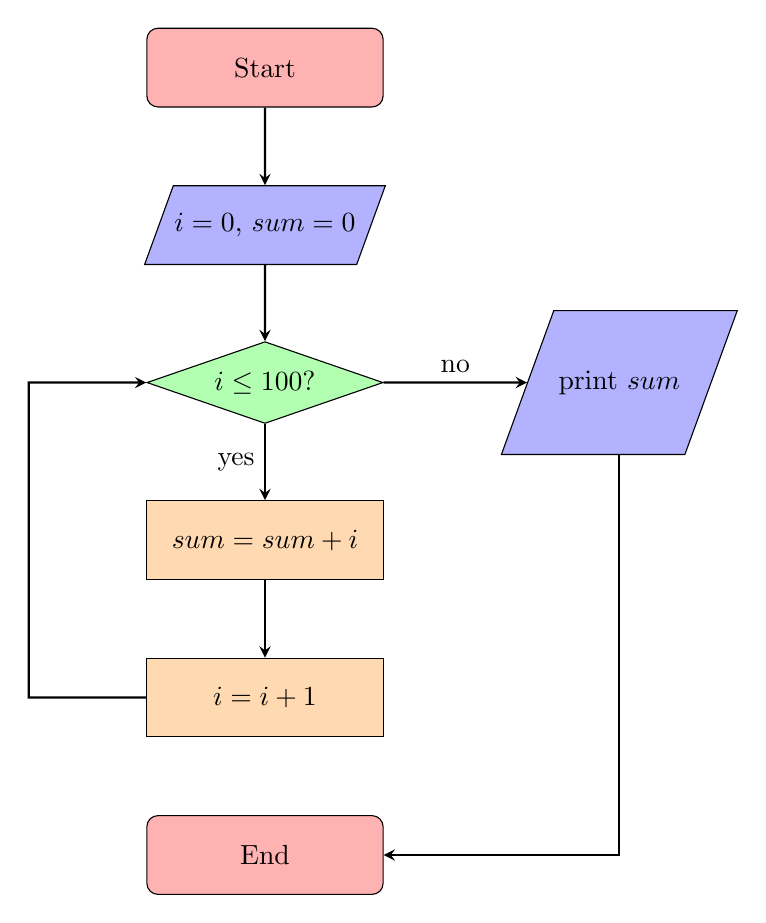
\begin{tikzpicture}[node distance=2cm]
		\node (start) [startend] {Start};
		\node (init) [io, below of=start] {$ i = 0 $, $ sum = 0 $};
		\node (decision)  [decision, below of=init] {$ i \le 100 $?};
		\node (accumulation) [process, below of=decision] {$ sum = sum + i $};
		\node (update) [process, below of=accumulation] {$ i = i + 1 $};
		\node (output) [io, right of=decision, xshift=2.5cm] {print $ sum $};
		\node (end) [startend, below of=update] {End};

		\draw [arrow] (start) -- (init);
		\draw [arrow] (init) -- (decision);
		\draw [arrow] (decision) -- node[anchor=east] {yes } (accumulation);
		\draw [arrow] (accumulation) -- (update);
		\draw [arrow] (update) -- (-3,-8) -- (-3,-4) -- (decision);
		\draw [arrow] (decision) -- node[anchor=south] {no} (output);
		\draw [arrow] (output) |- (end);
	\end{tikzpicture}
	\caption{计算$ \sum_{i=1}^{100} i $的流程图}
\end{figure}

\vspace{0.5cm}

\subsection{Hello World!}

Hello World是学习编程的第一个程序,它的作用是向屏幕输出"Hello World!"。\\

\mybox{Hello World!}

\begin{lstlisting}[language=C++]
#include <iostream>

using namespace std;

int main()
{
	cout << "Hello World!" << endl;
	return 0;
}
\end{lstlisting}

\begin{tcolorbox}
	\mybox{运行结果}
	\begin{verbatim}
Hello World!
	\end{verbatim}
\end{tcolorbox}

\#include <stdio.h>用于包含输入输出库的头文件(header file),这样才能够在程序中进行输入输出相关的操作。\\

using namespace std表示使用std命名空间。\\

main()是程序的入口,程序运行后会首先执行main()中的代码。cout的功能是在屏幕上输出数据,endl表示输出一个换行符。最后的分号用于表示一条语句的结束,注意不要使用中文的分号。\\

return 0表示main()运行结束,返回值为0,一般返回0用于表示程序正常结束。\\

不同编程语言的Hello World写法大同小异,可以看出编程语言的基本结构是相似的。\\

\mybox{C}

\begin{lstlisting}[language=C]
#include <stdio.h>

int main() {
	printf("Hello World!\n");
	return 0;
}
\end{lstlisting}

\vspace{0.5cm}

\mybox{Java}

\begin{lstlisting}[language=Java]
public class HelloWorld {
    public static void main(String[] args) {
        System.out.println("Hello World!");
    }
}
\end{lstlisting}

\vspace{0.5cm}

\mybox{Python}

\begin{lstlisting}[language=Python]
print("Hello World!")
\end{lstlisting}

\vspace{0.5cm}

\subsection{注释(Comment)}

注释就是对代码的解释和说明,它并不会程序所执行。注释能提高程序的可读性,让人更加容易了解代码的功能。\\

注释一般分为单行注释和多行注释:

\begin{enumerate}
	\item 单行注释:以//开头,该行之后的内容视为注释。
	\item 多行注释:以/*开头,*/结束,中间的内容视为注释。
\end{enumerate}

\vspace{0.5cm}

\mybox{注释}

\begin{lstlisting}[language=C++]
/*
* Author: Terry
* Date: 2022/11/16
*/

#include <iostream>      // header file

using namespace std;

int main()
{
	cout << "Hello World!" << endl;
	return 0;
}
\end{lstlisting}

\newpage

\section{数据类型}

\subsection{数据类型(Data Types)}

在计算机中,每个数据一般都有一个对应的类型,基础数据类型包括:

\begin{enumerate}
	\item 整型
	      \begin{itemize}
		      \item 短整型short
		      \item 整型int
		      \item 长整型long
		      \item 长长整型long long
	      \end{itemize}

	\item 浮点型
	      \begin{itemize}
		      \item 单精度浮点数float
		      \item 双精度浮点数double
	      \end{itemize}

	\item 字符型char
\end{enumerate}

\vspace{0.5cm}

不同的数据类型所占的内存空间大小不同,因此所能表示的数值范围也不同。\\

\begin{table}[H]
	\centering
	\setlength{\tabcolsep}{5mm}{
		\begin{tabular}{|c|c|c|}
			\hline
			\textbf{数据类型} & \textbf{大小} & \textbf{取值范围}           \\
			\hline
			short             & 2字节         & $ -2^{15} \sim 2^{15} - 1 $ \\
			\hline
			int               & 4字节         & $ -2^{31} \sim 2^{31} - 1 $ \\
			\hline
			long              & 4字节         & $ -2^{31} \sim 2^{31} - 1 $ \\
			\hline
			long long         & 8字节         & $ -2^{63} \sim 2^{63} - 1 $ \\
			\hline
			float             & 4字节         & 7位有效数字                 \\
			\hline
			double            & 8字节         & 15位有效数字                \\
			\hline
			char              & 1字节         & $ -128 \sim 127 $           \\
			\hline
		\end{tabular}
	}
\end{table}

\vspace{0.5cm}

\subsection{变量(Variable)}

变量是用来存储数据的内存空间,每个变量都有一个类型,变量中只能存储对应类型的数据。

\vspace{-0.5cm}

\begin{lstlisting}[language=C++]
int num = 10;
double salary = 8232.56;
\end{lstlisting}

\vspace{0.5cm}

变量的命名需要符合规范:

\begin{enumerate}
	\item 由字母、数字和下划线组成,不能以数字开头
	\item 不可以使用编程语言中预留的关键字
	\item 使用英语单词,顾名思义
\end{enumerate}

关键字是编程语言内置的一些名称,具有特殊的用处和意义,因此不应该作为变量名,防止产生歧义。\\

\begin{table}[H]
	\centering
	\setlength{\tabcolsep}{5mm}{
		\begin{tabular}{|c|c|c|c|c|}
			\hline
			asm      & auto     & break     & case     & catch    \\
			\hline
			char     & class    & const     & continue & default  \\
			\hline
			delete   & do       & double    & else     & enum     \\
			\hline
			extern   & float    & for       & friend   & goto     \\
			\hline
			if       & inline   & int       & long     & new      \\
			\hline
			operator & private  & protected & public   & register \\
			\hline
			return   & short    & signed    & sizeof   & static   \\
			\hline
			struct   & switch   & template  & this     & throw    \\
			\hline
			try      & typedef  & union     & unsigned & virtual  \\
			\hline
			void     & volatile & while     &          &          \\
			\hline
		\end{tabular}
	}
	\caption{关键字}
\end{table}

\vspace{0.5cm}

\subsection{常量(Constant)}

变量的值在程序运行过程中可以修改,但有一些数据的值是固定的,为了防止这些数据被随意改动,可以将这些数据定义为常量。\\

在数据类型前加上const关键字,即可定义常量,常量一般使用大写表示。如果在程序中尝试修改常量,将会报错。\\

\mybox{常量}

\begin{lstlisting}[language=C++]
#include <iostream>

using namespace std;

int main()
{
	const double PI = 3.1415;
	PI = 4;
	return 0;
}
\end{lstlisting}

\begin{tcolorbox}
	\mybox{运行结果}\\
	\textcolor{red}{error: assignment of read-only variable "PI"}
\end{tcolorbox}

\newpage

\section{输入输出}

\subsection{cout}

cout是输出流对象,用来向屏幕输出数据。但是有些需要输出的字符在编程语言中具有特殊含义,因此这些特殊的字符,需要经过转义后输出。\\

\begin{table}[H]
	\centering
	\setlength{\tabcolsep}{5mm}{
		\begin{tabular}{|c|c|}
			\hline
			\textbf{转义字符}      & \textbf{描述}                \\
			\hline
			\lstinline|\\| & 反斜杠\lstinline|\| \\
			\hline
			\lstinline|\'| & 单引号\lstinline|'| \\
			\hline
			\lstinline|\"| & 双引号\lstinline|"| \\
			\hline
			\lstinline|\n| & 换行                         \\
			\hline
			\lstinline|\t| & 制表符                       \\
			\hline
		\end{tabular}
	}
	\caption{转义字符}
\end{table}

\mybox{转义字符}

\begin{lstlisting}[language=C++]
#include <iostream>

using namespace std;

int main()
{
	cout << "\"Hello\nWorld\"" << endl;
	return 0;
}
\end{lstlisting}

\begin{tcolorbox}
	\mybox{运行结果}
	\begin{verbatim}
"Hello
World"
	\end{verbatim}
\end{tcolorbox}

在对变量的值进行输出时,可以使用格式控制符改变输出的格式。\\

\mybox{长方形面积}

\begin{lstlisting}[language=C++]
#include <iostream>
#include <iomanip>

using namespace std;

int main()
{
	int length = 10;
	int width = 5;
	double area = length * width;

	cout << "Area = " << length << " * " << width << " = "
			<< fixed << setprecision(2) << area << endl;
	return 0;
}
\end{lstlisting}

\begin{tcolorbox}
	\mybox{运行结果}
	\begin{verbatim}
Area = 10 * 5 = 50.00
	\end{verbatim}
\end{tcolorbox}

\vspace{0.5cm}

\subsection{printf()}

printf()是C语言中的输出函数,包含在头文件stdio.h中,用于向屏幕输出指定格式的文本,使用对应类型的占位符可以更加方便地输出变量的值。\\

\begin{table}[H]
	\centering
	\setlength{\tabcolsep}{5mm}{
		\begin{tabular}{|c|c|}
			\hline
			\textbf{数据类型} & \textbf{占位符} \\
			\hline
			int               & \%d             \\
			\hline
			float             & \%f             \\
			\hline
			double            & \%f             \\
			\hline
			char              & \%c             \\
			\hline
		\end{tabular}
	}
	\caption{占位符}
\end{table}

\vspace{-0.5cm}

\begin{lstlisting}[language=C]
printf("Area = %d * %d = %.2f\n", length, width, area);
\end{lstlisting}

\vspace{0.5cm}

\subsection{cin}

有时候一些数据需要从键盘输入,cin可以读取对应类型的数据,并赋值给相应的变量。\\

在使用cin前,通常会使用cout先输出一句提示信息,告诉用户需要输入什么数据。\\

\mybox{圆面积}

\begin{lstlisting}[language=C++]
#include <iostream>
#include <cmath>
#include <iomanip>

using namespace std;

int main()
{
	const double PI = 3.14159;
	double r;
	double area;

	cout << "Radius: ";
	cin >> r;

	area = PI * pow(r, 2);
	cout << "Area = " << fixed << setprecision(2) << area << endl;
	
	return 0;
}
\end{lstlisting}

\begin{tcolorbox}
	\mybox{运行结果}
	\begin{verbatim}
Radius: 5
Area = 78.54
	\end{verbatim}
\end{tcolorbox}

头文件cmath中定义了一些常用的数学函数,例如pow(x, y)可用于计算$ x $的$ y $次方。\\

\newpage

\section{表达式}

\subsection{算术运算符}

大部分编程语言中的除法与数学中的除法意义不同。\\

当相除的两个数都为整数时,那么就会进行整除运算,因此结果仍为整数,例如21 / 4 = 5。\\

如果相除的两个数中至少有一个为浮点数时,那么就会进行普通的除法运算,结果为浮点数,例如21.0 / 4 = 5.25。\\

取模(modulo)运算符\%用于计算两个整数相除之后的余数,例如22 \% 3 = 1、4 \% 7 = 4。\\

\mybox{逆序三位数}

\begin{lstlisting}[language=C++]
#include <iostream>

using namespace std;

int main()
{
	int num;
	int a, b, c;

	cout << "Enter a 3-digit integer: ";
	cin >> num;

	a = num / 100;
	b = num / 10 % 10;
	c = num % 10;

	cout << "Reversed: " << c*100 + b*10 + a << endl;
	return 0;
}
\end{lstlisting}

\begin{tcolorbox}
	\mybox{运行结果}
	\begin{verbatim}
Enter a 3-digit integer: 520
Reversed: 25
	\end{verbatim}
\end{tcolorbox}

\vspace{0.5cm}

\subsection{复合运算符}

使用复合运算符可以使表达式更加简洁。例如\lstinline|a = a + b|可以写成\lstinline|a += b|,-=、*=、/=、\%=等复合运算符的使用方式同理。\\

当需要给一个变量的值加/减1时,除了可以使用\lstinline|a += 1|或\lstinline|a -= 1|之外,还可以使用++或--运算符,但是\lstinline|++|和\lstinline|--|可以出现在变量之前或之后:\\

\begin{table}[H]
	\centering
	\setlength{\tabcolsep}{5mm}{
		\begin{tabular}{|c|l|}
			\hline
			\textbf{表达式}         & \textbf{含义}         \\
			\hline
			\lstinline|a++| & 执行完所在语句后自增1 \\
			\hline
			\lstinline|++a| & 在执行所在语句前自增1 \\
			\hline
			\lstinline|a--| & 执行完所在语句后自减1 \\
			\hline
			\lstinline|--a| & 在执行所在语句前自减1 \\
			\hline
		\end{tabular}
	}
	\caption{自增/自减运算符}
\end{table}

\mybox{自增/自减运算符}

\begin{lstlisting}[language=C++]
#include <iostream>

using namespace std;

int main()
{
	int n = 10;

	cout << n++ << endl;
	cout << ++n << endl;
	cout << n-- << endl;
	cout << --n << endl;

	return 0;
}
\end{lstlisting}

\begin{tcolorbox}
	\mybox{运行结果}
	\begin{verbatim}
10
12
12
10
	\end{verbatim}
\end{tcolorbox}

\vspace{0.5cm}

\subsection{隐式类型转换}

在计算机计算的过程中,只有类型相同的数据才可以进行运算。例如整数+整数、浮点数/浮点数等。\\

但是很多时候,我们仍然可以对不同类型的数据进行运算,而并不会产生错误,例如整数+浮点数。这是由于编译器会自动进行类型转换。在整数+浮点数的例子中,编译器会将整数转换为浮点数,这样就可以进行运算了。\\

编译器选择将整数转换为浮点数,而不是将浮点数转换为整数的原因在于,浮点数相比整数能够表示的范围更大。例如整数8可以使用8.0表示,而浮点数9.28变为整数9后就会丢失精度。\\

隐式类型转换最常见的情形就是除法运算,这也是导致整数/整数=整数、整数/浮点数=浮点数的原因。\\

\subsection{显式类型转换}

有些时候编译器无法自动进行类型转换,这时就需要我们手动地强制类型转换。\\

\mybox{显式类型转换}

\begin{lstlisting}[language=C++]
#include <iostream>
#include <iomanip>

using namespace std;

int main()
{
	int total = 821;
	int num = 10;
	double average = (double)total / num;
	cout << "Average = " << fixed << setprecision(2) << average << endl;
	return 0;
}
\end{lstlisting}

\begin{tcolorbox}
	\mybox{运行结果}
	\begin{verbatim}
Average = 82.10
	\end{verbatim}
\end{tcolorbox}

\newpage
\chapter{分支}

\section{逻辑运算符}

\subsection{关系运算符}

编程中经常需要使用关系运算符来比较两个数据的大小,比较的结果是一个布尔值(boolean),即True(非0)或False(0)。\\

在编程中需要注意,一个等号=表示赋值运算,而两个等号==表示比较运算。\\

\begin{table}[H]
	\centering
	\setlength{\tabcolsep}{5mm}{
		\begin{tabular}{|c|c|}
			\hline
			\textbf{数学符号} & \textbf{关系运算符} \\
			\hline
			$ < $             & <                   \\
			\hline
			$ > $             & >                   \\
			\hline
			$ \le $           & <=                  \\
			\hline
			$ \ge $           & >=                  \\
			\hline
			$ = $             & ==                  \\
			\hline
			$ \ne $           & !=                  \\
			\hline
		\end{tabular}
	}
\end{table}

\vspace{0.5cm}

\subsection{逻辑运算符}

逻辑运算符用于连接多个关系表达式,其结果也是一个布尔值。\\

\begin{enumerate}
	\item 逻辑与\&\&:当多个条件全部为True,结果为True。\\
	      \begin{table}[H]
		      \centering
		      \setlength{\tabcolsep}{5mm}{
			      \begin{tabular}{|c|c|c|}
				      \hline
				      \textbf{条件1} & \textbf{条件2} & \textbf{条件1 \&\& 条件2} \\
				      \hline
				      T              & T              & T                         \\
				      \hline
				      T              & F              & F                         \\
				      \hline
				      F              & T              & F                         \\
				      \hline
				      F              & F              & F                         \\
				      \hline
			      \end{tabular}
		      }
	      \end{table}

	\item 逻辑或||:多个条件至少有一个为True时,结果为True。\\
	      \begin{table}[H]
		      \centering
		      \setlength{\tabcolsep}{5mm}{
			      \begin{tabular}{|c|c|c|}
				      \hline
				      \textbf{条件1} & \textbf{条件2} & \textbf{条件1 || 条件2} \\
				      \hline
				      T              & T              & T                       \\
				      \hline
				      T              & F              & T                       \\
				      \hline
				      F              & T              & T                       \\
				      \hline
				      F              & F              & F                       \\
				      \hline
			      \end{tabular}
		      }
	      \end{table}

	\item 逻辑非!:条件为True时,结果为False;条件为False时,结果为True。\\
	      \begin{table}[H]
		      \centering
		      \setlength{\tabcolsep}{5mm}{
			      \begin{tabular}{|c|c|}
				      \hline
				      \textbf{条件} & \textbf{!条件} \\
				      \hline
				      T             & F              \\
				      \hline
				      F             & T              \\
				      \hline
			      \end{tabular}
		      }
	      \end{table}
\end{enumerate}

\newpage

\section{if}

\subsection{if}

if语句用于判断一个条件是否成立,如果成立则进入语句块,否则不执行。\\

\mybox{年龄}

\begin{lstlisting}[language=C++]
#include <iostream>

using namespace std;

int main()
{
	int age;
	cout << "Enter your age: ";
	cin >> age;
	if(age > 0 && age < 18)
	{
		cout << "Minor" << endl;
	}
	return 0;
}
\end{lstlisting}

\begin{tcolorbox}
	\mybox{运行结果}
	\begin{verbatim}
Enter your age: 17
Minor
\end{verbatim}
\end{tcolorbox}

\vspace{0.5cm}

\subsection{if-else}

if-else的结构与if类似,只是在if语句块中的条件不成立时,执行else语句块中的语句。\\

\mybox{闰年}

\begin{lstlisting}[language=C++]
#include <iostream>

using namespace std;

int main()
{
	int year;
	cout << "Enter a year: ";
	cin >> year;

	/*
		* A year is a leap year if it is
		* 1. exactly divisible by 4, and not divisible by 100;
		* 2. or is exactly divisible by 400
		*/
	if((year % 4 == 0 && year % 100 != 0) || year % 400 == 0)
	{
		cout << "Leap year" << endl;
	}
	else
	{
		cout << "Common year" << endl;
	}

	return 0;
}
\end{lstlisting}

\begin{tcolorbox}
	\mybox{运行结果}
	\begin{verbatim}
Enter a year: 2020
Leap year
\end{verbatim}
\end{tcolorbox}

\vspace{0.5cm}

\subsection{if-else if-else}

当需要对更多的条件进行判断时,可以使用if-else if-else语句。\\

\mybox{字符}

\begin{lstlisting}[language=C++]
#include <iostream>

using namespace std;

int main()
{
	char c;
	cout << "Enter a character: ";
	cin >> c;

	if(c >= 'a' && c <= 'z')
	{
		cout << "Lowercase" << endl;
	}
	else if(c >= 'A' && c <= 'Z')
	{
		cout << "Uppercase" << endl;
	}
	else if(c >= '0' && c <= '9')
	{
		cout << "Digit" << endl;
	}
	else
	{
		cout << "Special character" << endl;
	}
	
	return 0;
}
\end{lstlisting}

\begin{tcolorbox}
	\mybox{运行结果}
	\begin{verbatim}
Enter a character: T
Uppercase
\end{verbatim}
\end{tcolorbox}

\newpage

\section{switch}

\subsection{switch}

switch结构用于根据一个整数值,选择对应的case执行。需要注意的是,当对应的case中的代码被执行完后,并不会像if语句一样跳出switch结构,而是会继续向后执行,直到遇到break。\\

\mybox{计算器}

\begin{lstlisting}[language=C++]
#include <iostream>

using namespace std;

int main() {
	int num1, num2;
	char op;

	cout << "Enter an expression: ";
	cin >> num1 >> op >> num2;

	switch (op)
	{
	case '+':
		cout << num1 << " + " << num2 << " = " << num1 + num2 << endl;
		break;
	case '-':
		cout << num1 << " - " << num2 << " = " << num1 - num2 << endl;
		break;
	case '*':
		cout << num1 << " * " << num2 << " = " << num1 * num2 << endl;
		break;
	case '/':
		cout << num1 << " / " << num2 << " = " << num1 / num2 << endl;
		break;
	default:
		cout << "Error! Operator is not supported" << endl;
		break;
	}

	return 0;
}
\end{lstlisting}

\begin{tcolorbox}
	\mybox{运行结果}
	\begin{verbatim}
Enter an expression: 5 * 8
5 * 8 = 40
\end{verbatim}
\end{tcolorbox}

\newpage
\chapter{循环}

\section{while}

\subsection{while}

while循环会对条件进行判断,如果条件成立,就会执行循环体,然后再次判断条件,直到条件不成立。\\

while循环的次数由循环变量的变化决定,因此while循环一般都包括对循环变量的初值、判断和更新。

\vspace{-0.5cm}

\begin{lstlisting}[language=C++]
int i = 1;          // initial value
while(i <= 5)       // condition
{
    cout << "In loop: i = " << i << endl;
    i++;            // update
}
cout << "After loop: i = " << i << endl;
\end{lstlisting}

while循环的特点是先判断、再执行,因此循环体有可能会执行一次或多次,也有可能一次也不会执行。\\

\mybox{平均身高}

\begin{lstlisting}[language=C++]
#include <iostream>
#include <iomanip>

#define NUM_PEOPLE 5

using namespace std;

int main()
{
    double height;
    double total = 0;

    int i = 1;
    while (i <= NUM_PEOPLE)
    {
        cout << "Enter person " << i << "'s height: ";
        cin >> height;
        total += height;
        i++;
    }

    double average = total / NUM_PEOPLE;
    cout << "Average height: "
         << fixed << setprecision(2) << average << endl;
    
    return 0;
}
\end{lstlisting}

\begin{tcolorbox}
    \mybox{运行结果}
    \begin{verbatim}
Enter person 1's height: 160.8
Enter person 2's height: 175.2
Enter person 3's height: 171.2
Enter person 4's height: 181.3
Enter person 5's height: 164
Average height: 170.50
\end{verbatim}
\end{tcolorbox}

\vspace{0.5cm}

\mybox{统计元音、辅音数量}

\begin{lstlisting}[language=C++]
#include <iostream>

using namespace std;

int main()
{
    char c;
    int vowel = 0;
    int consonant = 0;

    cout << "Enter an English sentence: ";

    while((c = cin.get()) != '\n')
    {
        if (c == 'a' || c == 'A' ||
            c == 'e' || c == 'E' || 
            c == 'i' || c == 'I' || 
            c == 'o' || c == 'O' || 
            c == 'u' || c == 'U')
        {
            vowel++;
        }
        else if ((c >= 'a' && c <= 'z') || (c >= 'A' && c <= 'Z'))
        {
            consonant++;
        }
    }

    cout << "Vowel = " << vowel << endl;
    cout << "Consonant = " << consonant << endl;
    return 0;
}
\end{lstlisting}

\begin{tcolorbox}
    \mybox{运行结果}
    \begin{verbatim}
Enter an English sentence: Hello World!
Vowel = 3
Consonant = 7
\end{verbatim}
\end{tcolorbox}

\vspace{0.5cm}

\subsection{do-while}

do-while循环是先执行一轮循环体内的代码后,再检查循环的条件是否成立。如果成立,则继续下一轮循环;否则循环结束。\\

do-while循环是先执行、再判断,因此它至少会执行一轮循环。do-while一般应用在一些可能会需要重复,但必定会发生一次的情景下。例如登录账户,用户输入账户和密码后,检查是否正确,如果正确,那么就成功登录;否则继续循环让用户重新输入。\\

需要注意,do-while循环的最后有一个分号。

\vspace{-0.5cm}

\begin{lstlisting}[language=C++]
do {
    // code
} while(condition);
\end{lstlisting}

\vspace{0.5cm}

\mybox{整数位数}

\begin{lstlisting}[language=C++]
#include <iostream>

using namespace std;

int main()
{
    int num;
    int n = 0;

    cout << "Enter an integer: ";
    cin >> num;

    do
    {
        num /= 10;
        n++;
    } while(num != 0);

    cout << "Digits: " << n << endl;
    return 0;
}
\end{lstlisting}

\begin{tcolorbox}
    \mybox{运行结果}
    \begin{verbatim}
Enter an integer: 123
Digits: 3
\end{verbatim}
\end{tcolorbox}

\vspace{0.5cm}

\mybox{猜数字}

\begin{lstlisting}[language=C++]
#include <iostream>
#include <cstdlib>
#include <ctime>

using namespace std;

int main()
{
    srand(time(NULL));          // set random seed

    // generate random number between 1 and 100
    int answer = rand() % 100 + 1;
    int num = 0;
    int cnt = 0;

    do
    {
        cout << "Guess a number: ";
        cin >> num;
        cnt++;
        
        if(num > answer)
        {
            cout << "Too high" << endl;
        }
        else if(num < answer)
        {
            cout << "Too low" << endl;
        }
    } while(num != answer);

    cout << "Correct! You guessed " << cnt << " times." << endl;
    return 0;
}
\end{lstlisting}

\begin{tcolorbox}
    \mybox{运行结果}
    \begin{verbatim}
Guess a number: 50
Too high
Guess a number: 25
Too low
Guess a number: 37
Too low
Guess a number: 43
Too high
Guess a number: 40
Too high
Guess a number: 38
Too low
Guess a number: 39
Correct! You guessed 7 times.
\end{verbatim}
\end{tcolorbox}

\newpage

\section{for}

\subsection{for}

while循环将循环变量的初值、条件和更新写在了三个地方,但是这样不容易明显地看出循环变量的变化。\\

for循环将循环变量的初值、条件和更新写在了一行内,中间用分号隔开。对于指定次数的循环一般更多地会采用for循环,而对于不确定次数的一般会采用while循环。

\vspace{-0.5cm}

\begin{lstlisting}[language=C++]
for(int i = 0; i < 5; i++)
{
    cout << "i = " << i << endl;
}
\end{lstlisting}

\vspace{0.5cm}

\mybox{累加}

\begin{lstlisting}[language=C++]
#include <iostream>

using namespace std;

int main()
{
    int sum = 0;
    for(int i = 1; i <= 100; i++)
    {
        sum += i;
    }
    cout << "Sum = " << sum << endl;
    return 0;
}
\end{lstlisting}

\begin{tcolorbox}
    \mybox{运行结果}
    \begin{verbatim}
Sum = 5050
\end{verbatim}
\end{tcolorbox}

\vspace{0.5cm}

\mybox{斐波那契数列}

\begin{figure}[H]
    \centering
    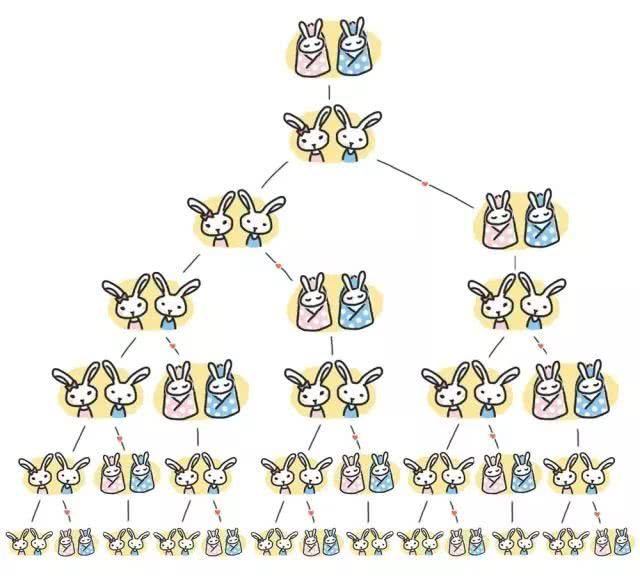
\includegraphics[scale=0.5]{img/Chapter3/3-2/1.png}
\end{figure}

\begin{lstlisting}[language=C++]
#include <iostream>

using namespace std;

int main()
{
    int n;
    cout << "Enter the number of terms: ";
    cin >> n;

    if(n == 1)
    {
        cout << "1" << endl;
    }
    else if(n == 2)
    {
        cout << "1, 1" << endl;
    }
    else
    {
        int num1, num2, val;
        num1 = 1;
        num2 = 1;
        cout << "1, 1";

        for(int i = 3; i <= n; i++)
        {
            val = num1 + num2;
            cout << ", " << val;
            num1 = num2;
            num2 = val;
        }
        cout << endl;
    }
    
    return 0;
}
\end{lstlisting}

\begin{tcolorbox}
    \mybox{运行结果}
    \begin{verbatim}
Enter the number of terms: 10
1, 1, 2, 3, 5, 8, 13, 21, 34, 55
\end{verbatim}
\end{tcolorbox}

\vspace{0.5cm}

\subsection{嵌套循环}

循环也可以嵌套使用,外层循环每执行一次,内层循环就会执行多次。

\vspace{-0.5cm}

\begin{lstlisting}[language=C++]
for(int i = 0; i < 2; i++)
{
    for(int j = 0; j < 3; j++)
    {
        cout << "i = " << i << ", j = " << j << endl;
    }
}
\end{lstlisting}

\begin{tcolorbox}
    \mybox{运行结果}
    \begin{verbatim}
i = 0, j = 0
i = 0, j = 1
i = 0, j = 2
i = 1, j = 0
i = 1, j = 1
i = 1, j = 2
\end{verbatim}
\end{tcolorbox}

\vspace{0.5cm}

\mybox{九九乘法表}\\

\begin{table}[H]
    \centering
    \setlength{\tabcolsep}{1.5mm}{
        \begin{tabular}{|c|c|c|c|c|c|c|c|c|}
            \hline
            1*1=1 & 1*2=2  & 1*3=3  & 1*4=4  & 1*5=5  & 1*6=6  & 1*7=7  & 1*8=8  & 1*9=9  \\
            \hline
            2*1=2 & 2*2=4  & 2*3=6  & 2*4=8  & 2*5=10 & 2*6=12 & 2*7=14 & 2*8=16 & 2*9=18 \\
            \hline
            3*1=3 & 3*2=6  & 3*3=9  & 3*4=12 & 3*5=15 & 3*6=18 & 3*7=21 & 3*8=24 & 3*9=27 \\
            \hline
            4*1=4 & 4*2=8  & 4*3=12 & 4*4=16 & 4*5=20 & 4*6=24 & 4*7=28 & 4*8=32 & 4*9=36 \\
            \hline
            5*1=5 & 5*2=10 & 5*3=15 & 5*4=20 & 5*5=25 & 5*6=30 & 5*7=35 & 5*8=40 & 5*9=45 \\
            \hline
            6*1=6 & 6*2=12 & 6*3=18 & 6*4=24 & 6*5=30 & 6*6=36 & 6*7=42 & 6*8=48 & 6*9=54 \\
            \hline
            7*1=7 & 7*2=14 & 7*3=21 & 7*4=28 & 7*5=35 & 7*6=42 & 7*7=49 & 7*8=56 & 7*9=63 \\
            \hline
            8*1=8 & 8*2=16 & 8*3=24 & 8*4=32 & 8*5=40 & 8*6=48 & 8*7=56 & 8*8=64 & 8*9=72 \\
            \hline
            9*1=9 & 9*2=18 & 9*3=27 & 9*4=36 & 9*5=45 & 9*6=54 & 9*7=63 & 9*8=72 & 9*9=81 \\
            \hline
        \end{tabular}
    }
\end{table}

\begin{lstlisting}[language=C++]
#include <iostream>

using namespace std;

int main()
{
    for(int i = 1; i <= 9; i++)
    {
        for(int j = 1; j <= 9; j++)
        {
            cout << i << "*" << j << "=" << i*j << "\t";
        }
        cout << endl;
    }
    return 0;
}
\end{lstlisting}

\vspace{0.5cm}

\mybox{打印图案}

\begin{lstlisting}
*
**
***
****
*****
\end{lstlisting}

\begin{lstlisting}[language=C++]
#include <iostream>

using namespace std;

int main()
{
    for(int i = 1; i <= 5; i++)
    {
        for(int j = 1; j <= i; j++)
        {
            cout << "*";
        }
        cout << endl;
    }
    return 0;
}
\end{lstlisting}

\newpage

\section{break or continue?}

\subsection{break}

break可用于跳出当前的switch或循环结构。在一些情况下,在循环的中途已经完成了某个目标,没有必要再进行剩余的循环,这时就可以使用break跳出循环。\\

例如在判断一个数$ n $是否为素数时,利用循环逐个判断$ 2 \sim n - 1 $之间的数是否能整除$ n $。只要发现其中有一个数能整除$ n $,就证明$ n $不是素数,可以跳出循环,不必再进行剩余的检查。\\

\mybox{素数}

\begin{lstlisting}[language=C++]
#include <iostream>
#include <cmath>

using namespace std;

int main()
{
    int n;
    cout << "Enter an integer: ";
    cin >> n;

    bool is_prime = true;
    for(int i = 2; i <= sqrt(n); i++)
    {
        if(n % i == 0)
        {
            is_prime = false;
            break;
        }
    }

    if(is_prime)
    {
        cout << n << " is a prime number" << endl;
    }
    else
    {
        cout << n << " is not a prime number" << endl;
    }

    return 0;
}
\end{lstlisting}

\begin{tcolorbox}
    \mybox{运行结果}
    \begin{verbatim}
Enter an integer: 17
17 is a prime number
\end{verbatim}
\end{tcolorbox}

\vspace{0.5cm}

\subsection{continue}

continue与break使用方法类似,但是它并不是跳出循环,而是跳过本轮循环,直接开始下一轮循环。\\

\mybox{正数平方和}

\begin{lstlisting}[language=C]
#include <iostream>

using namespace std;

int main()
{
    int n = 10;
    cout << "Enter " << n << " integers: ";

    int sum_square = 0;
    for(int i = 0; i < n; i++)
    {
        int num;
        cin >> num;
        if(num < 0)
        {
            continue;
        }

        sum_square += num * num;
    }

    cout << "Sum of squares of positive integers: "
            << sum_square << endl;
            
    return 0;
}
\end{lstlisting}

\begin{tcolorbox}
    \mybox{运行结果}
    \begin{verbatim}
Enter 10 integers: 5 7 -2 0 4 -4 -9 3 9 5
Sum of squares of positive integers: 205
\end{verbatim}
\end{tcolorbox}

\newpage
\chapter{数组}

\section{数组}

\subsection{数组(Array)}

数组能够存储一组类型相同的元素,数组在声明时必须指定它的大小(容量),数组的大小是固定的,无法在运行时动态改变。数组通过下标(index)来访问某一位置上的元素,下标从0开始。

\vspace{-0.5cm}

\begin{lstlisting}[language=C]
int arr[5] = {3, 6, 8, 2, 4};
\end{lstlisting}

\begin{figure}[H]
	\centering
	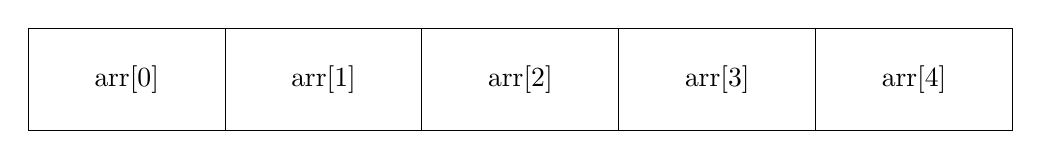
\begin{tikzpicture}[scale=0.5]
		\draw[-] (0,0) -- (5,0) -- (10,0) -- (15,0) -- (20,0) -- (25,0) -- (25,2.6) -- (20,2.6) -- (15,2.6) -- (10,2.6) -- (5,2.6) -- (0,2.6) -- (0,0);
		\draw[-] (5,0) -- (5,2.6);
		\draw[-] (10,0) -- (10,2.6);
		\draw[-] (15,0) -- (15,2.6);
		\draw[-] (20,0) -- (20,2.6);

		\draw (2.5,1.3) node {arr[0]};
		\draw (7.5,1.3) node {arr[1]};
		\draw (12.5,1.3) node {arr[2]};
		\draw (17.5,1.3) node {arr[3]};
		\draw (22.5,1.3) node {arr[4]};
	\end{tikzpicture}
\end{figure}

如果在声明数组时没有指定数组的大小,那么将根据初始化的元素个数来确定。

\vspace{-0.5cm}

\begin{lstlisting}[language=C]
int arr[] = {3, 6, 8, 2, 4, 0, 1, 7};
\end{lstlisting}

通过下标可以访问数组中的元素,下标的有效范围是0 $ \sim $ 数组的长度 - 1,如果使用不合法的下标就会导致数组越界。

\vspace{-0.5cm}

\begin{lstlisting}[language=C]
printf("%d\n", arr[0]);		// 3
printf("%d\n", arr[3]);		// 2
printf("%d\n", arr[7]);		// 7
\end{lstlisting}

当数组的容量比较大时,可以使用循环来初始化数组。

\vspace{-0.5cm}

\begin{lstlisting}[language=C]
int arr[10];

for(int i = 0; i < 10; i++) {
	arr[i] = i + 1;
}
\end{lstlisting}

\vspace{0.5cm}

\mybox{查找数据}

\begin{lstlisting}[language=C]
#include <stdio.h>
#include <stdbool.h>

int main() {
	int n;
	printf("Enter the number of elements: ");
	scanf("%d", &n);

	int arr[n];
	printf("Enter the elements: ");
	for (int i = 0; i < n; i++) {
		scanf("%d", &arr[i]);
	}

	int key;
	printf("Enter the key: ");
	scanf("%d", &key);

	bool found = false;
	for (int i = 0; i < n; i++) {
		if (arr[i] == key) {
			found = true;
			break;
		}
	}

	if (found) {
		printf("%d exists.\n", key);
	} else {
		printf("%d not found!\n", key);
	}

	return 0;
}
\end{lstlisting}

\begin{tcolorbox}
	\mybox{运行结果}
	\begin{verbatim}
Enter the number of elements: 5
Enter the elements: 4 8 9 2 3
Enter the key: 2
2 exists.
	\end{verbatim}
\end{tcolorbox}

\vspace{0.5cm}

\mybox{最大值/最小值}

\begin{lstlisting}[language=C]
#include <stdio.h>

int main() {
	int num[] = {7, 6, 2, 9, 3, 1, 4, 0, 5, 8};
	int n = sizeof(num) / sizeof(num[0]);
	int max = num[0];
	int min = num[0];

	for(int i = 1; i < n; i++) {
		if(num[i] > max) {
			max = num[i];
		}
		if(num[i] < min) {
			min = num[i];
		}
	}

	printf("Max = %d\n", max);
	printf("Min = %d\n", min);
	return 0;
}
\end{lstlisting}

\begin{tcolorbox}
	\mybox{运行结果}
	\begin{verbatim}
Max = 9
Min = 0
	\end{verbatim}
\end{tcolorbox}

\vspace{0.5cm}

\subsection{二维数组(2-Dimensional Array)}

二维数组由行和列两个维度组成,行和列的下标同样也都是从0开始。在声明二维数组时,需要指定行和列的大小。二维数组可以看成是由多个一维数组组成的,因此二维数组中的每个元素都是一个一维数组。

\vspace{-0.5cm}

\begin{lstlisting}[language=C]
int arr[3][4] = {{1, 2, 3, 4}, {5, 6, 7, 8}, {9, 10, 11, 12}};
\end{lstlisting}

\begin{table}[H]
	\centering
	\setlength{\tabcolsep}{5mm}{
		\begin{tabular}{|c|c|c|c|}
			\hline
			arr[0][0] & arr[0][1] & arr[0][2] & arr[0][3] \\
			\hline
			arr[1][0] & arr[1][1] & arr[1][2] & arr[1][3] \\
			\hline
			arr[2][0] & arr[2][1] & arr[2][2] & arr[2][3] \\
			\hline
		\end{tabular}
	}
\end{table}

在初始化二维数组时,为了能够更直观地看出二维数组的结构,可以将每一行单独写在一行中。

\vspace{-0.5cm}

\begin{lstlisting}[language=C]
int arr[3][4] = {
	{1, 2, 3, 4},
	{5, 6, 7, 8},
	{9, 10, 11, 12},
};
\end{lstlisting}

对于容量较大的二维数组,可以通过两层循环进行初始化。

\vspace{-0.5cm}

\begin{lstlisting}[language=C]
int arr[3][4];

for(int i = 0; i < 3; i++) {
	for(int j = 0; j < 4; j++) {
		arr[i][j] = 0;
	}
}
\end{lstlisting}

\vspace{0.5cm}

\mybox{矩阵运算}

\begin{align}\nonumber
	\left[\begin{matrix}
			1 & 3 \\
			1 & 0 \\
			1 & 2 \\
		\end{matrix} \right]
	+
	\left[\begin{matrix}
			0 & 0 \\
			7 & 5 \\
			2 & 1 \\
		\end{matrix} \right]
	=
	\left[\begin{matrix}
			1+0 & 3+0 \\
			1+7 & 0+5 \\
			1+2 & 2+1 \\
		\end{matrix} \right]
	=
	\left[\begin{matrix}
			1 & 3 \\
			8 & 5 \\
			3 & 3 \\
		\end{matrix} \right]
\end{align}

\begin{align}\nonumber
	\left[\begin{matrix}
			1 & 3 \\
			1 & 0 \\
			1 & 2 \\
		\end{matrix} \right]
	-
	\left[\begin{matrix}
			0 & 0 \\
			7 & 5 \\
			2 & 1 \\
		\end{matrix} \right]
	=
	\left[\begin{matrix}
			1-0 & 3-0 \\
			1-7 & 0-5 \\
			1-2 & 2-1 \\
		\end{matrix} \right]
	=
	\left[\begin{matrix}
			1  & 3  \\
			-6 & -5 \\
			-1 & 1  \\
		\end{matrix} \right]
\end{align}

\begin{lstlisting}[language=C]
#include <stdio.h>

int main() {
	int A[3][2] = {
		{1, 3},
		{1, 0},
		{1, 2}
	};
	int B[3][2] = {
		{0, 0},
		{7, 5},
		{2, 1}
	};
	int C[3][2];

	printf("Matrix Addition\n");
	for(int i = 0; i < 3; i++) {
		for(int j = 0; j < 2; j++) {
			C[i][j] = A[i][j] + B[i][j];
			printf("%3d", C[i][j]);
		}
		printf("\n");
	}
	
	printf("Matrix Subtraction\n");
	for(int i = 0; i < 3; i++) {
		for(int j = 0; j < 2; j++) {
			C[i][j] = A[i][j] - B[i][j];
			printf("%3d", C[i][j]);
		}
		printf("\n");
	}
	
	return 0;
}
\end{lstlisting}

\begin{tcolorbox}
	\mybox{运行结果}
	\begin{verbatim}
Matrix Addition
  1  3
  8  5
  3  3
Matrix Subtraction
  1  3
  -6 -5
  -1  1
	\end{verbatim}
\end{tcolorbox}

\newpage

\section{字符串}

\subsection{ASCII}

美国信息交换标准代码ASCII(American Standard Code for Information Interchange)一共定义了128个字符。\\

\begin{longtable}{|c|c|c|c|c|c|c|c|}
	\hline
	\textbf{ASCII} & \textbf{字符} & \textbf{ASCII} & \textbf{字符} & \textbf{ASCII} & \textbf{字符}          & \textbf{ASCII} & \textbf{字符}          \\
	\hline
	0              & NUT           & 32             & (space)       & 64             & @                      & 96             & \lstinline|`| \\
	\hline
	1              & SOH           & 33             & !             & 65             & A                      & 97             & a                      \\
	\hline
	2              & STX           & 34             & \text{"}      & 66             & B                      & 98             & b                      \\
	\hline
	3              & ETX           & 35             & \#            & 67             & C                      & 99             & c                      \\
	\hline
	4              & EOT           & 36             & \$            & 68             & D                      & 100            & d                      \\
	\hline
	5              & ENQ           & 37             & \%            & 69             & E                      & 101            & e                      \\
	\hline
	6              & ACK           & 38             & \&            & 70             & F                      & 102            & f                      \\
	\hline
	7              & BEL           & 39             & \text{'}      & 71             & G                      & 103            & g                      \\
	\hline
	8              & BS            & 40             & (             & 72             & H                      & 104            & h                      \\
	\hline
	9              & HT            & 41             & )             & 73             & I                      & 105            & i                      \\
	\hline
	10             & LF            & 42             & *             & 74             & J                      & 106            & j                      \\
	\hline
	11             & VT            & 43             & +             & 75             & K                      & 107            & k                      \\
	\hline
	12             & FF            & 44             & ,             & 76             & L                      & 108            & l                      \\
	\hline
	13             & CR            & 45             & -             & 77             & M                      & 109            & m                      \\
	\hline
	14             & SO            & 46             & .             & 78             & N                      & 110            & n                      \\
	\hline
	15             & SI            & 47             & /             & 79             & O                      & 111            & o                      \\
	\hline
	16             & DLE           & 48             & 0             & 80             & P                      & 112            & p                      \\
	\hline
	17             & DC1           & 49             & 1             & 81             & Q                      & 113            & q                      \\
	\hline
	18             & DC2           & 50             & 2             & 82             & R                      & 114            & r                      \\
	\hline
	19             & DC3           & 51             & 3             & 83             & S                      & 115            & s                      \\
	\hline
	20             & DC4           & 52             & 4             & 84             & T                      & 116            & t                      \\
	\hline
	21             & NAK           & 53             & 5             & 85             & U                      & 117            & u                      \\
	\hline
	22             & SYN           & 54             & 6             & 86             & V                      & 118            & v                      \\
	\hline
	23             & TB            & 55             & 7             & 87             & W                      & 119            & w                      \\
	\hline
	24             & CAN           & 56             & 8             & 88             & X                      & 120            & x                      \\
	\hline
	25             & EM            & 57             & 9             & 89             & Y                      & 121            & y                      \\
	\hline
	26             & SUB           & 58             & :             & 90             & Z                      & 122            & z                      \\
	\hline
	27             & ESC           & 59             & ;             & 91             & [                      & 123            & \{                     \\
			\hline
	28             & FS            & 60             & <             & 92             & $ \backslash $         & 124            & |                      \\
			\hline
	29             & GS            & 61             & =             & 93             & ]                      & 125            & \}                     \\
	\hline
	30             & RS            & 62             & >             & 94             & \lstinline|^| & 126            & \lstinline|~| \\
	\hline
	31             & US            & 63             & ?             & 95             & \_                     & 127            & DEL                    \\
	\hline
\end{longtable}

\vspace{0.5cm}

\mybox{ASCII}

\begin{lstlisting}[language=C]
#include <stdio.h>

int main() {
	for(int i = 0; i < 128; i++) {
		printf("%d - %c\n", i, i);
	}
	return 0;
}
\end{lstlisting}

\vspace{0.5cm}

\subsection{字符串(String)}

字符数组通常被称为字符串,字符串有两种初始化的方式。一种与普通数组的初始化类似,逐个写出每一个字符,最后需要手动添加$ \backslash $0字符,表示字符串的结束符;另一种是直接使用双引号,这种写法无需手动添加$ \backslash $0。

\vspace{-0.5cm}

\begin{lstlisting}[language=C]
char str[8] = {'p', 'r', 'o', 'g', 'r', 'a', 'm', '\0'};
char str[8] = "program";
\end{lstlisting}

$ \backslash $0占一个字符的大小,因此在设置字符串的大小时需要考虑$ \backslash $0。\\

占位符\%s可以对字符串进行输入输出操作,使用scanf()和gets()都可以用于读取字符串,但是scanf()只会读取到空格为止,而gets()会读取到回车为止。\\

\mybox{字符串输入输出}

\begin{lstlisting}[language=C]
#include <stdio.h>

int main() {
	char str1[32];
	printf("Enter string 1: ");
	gets(str1);
	puts(str1);

	char str2[32];
	printf("Enter string 2: ");
	scanf("%s", str2);
	printf("%s\n", str2);

	return 0;
}
\end{lstlisting}

\begin{tcolorbox}
	\mybox{运行结果}
	\begin{verbatim}
Enter string 1: hello world
hello world
Enter string 2: hello world
hello
	\end{verbatim}
\end{tcolorbox}

\vspace{0.5cm}

\mybox{字符统计}

\begin{lstlisting}[language=C]
#include <stdio.h>

int main() {
	char str[32];
	printf("Enter a string: ");
	gets(str);
	printf("Character to search: ");
	char c = getchar();

	int cnt = 0;
	int i = 0;
	while (str[i] != '\0') {
		if (str[i] == c) {
			cnt++;
		}
		i++;
	}

	printf("\'%c\' appears %d times in \"%s\".\n", c, cnt, str);
	return 0;
}
\end{lstlisting}

\begin{tcolorbox}
	\mybox{运行结果}
	\begin{verbatim}
Enter a string: this is a test
Character to search: t
't' appears 3 times in "this is a test".
	\end{verbatim}
\end{tcolorbox}

\vspace{0.5cm}

\subsection{字符串函数}

头文件<string.h>中定义了一些常用的字符串处理函数。

\subsubsection{strlen()}

计算字符串的长度。\\

\mybox{strlen()}

\begin{lstlisting}[language=C]
#include <stdio.h>
#include <string.h>

int main() {
	char s[] = "hello world";
	printf("Length: %d\n", strlen(s));
	return 0;
}
\end{lstlisting}

\begin{tcolorbox}
	\mybox{运行结果}
	\begin{verbatim}
Length: 11
	\end{verbatim}
\end{tcolorbox}

\vspace{0.5cm}

\subsubsection{strcpy()}

字符串复制,调用者需要确保字符串的大小足够。\\

\mybox{strcpy()}

\begin{lstlisting}[language=C]
#include <stdio.h>
#include <string.h>

int main() {
	char s1[32] = "hello world";
	char s2[32] = "program";

	strcpy(s1, s2);
	printf("s1 = %s\n", s1);
	printf("s2 = %s\n", s2);
	return 0;
}
\end{lstlisting}

\begin{tcolorbox}
	\mybox{运行结果}
	\begin{verbatim}
s1 = program
s2 = program
	\end{verbatim}
\end{tcolorbox}

\vspace{0.5cm}

\subsubsection{strcat()}

字符串拼接,调用者需要确保字符串的大小足够。\\

\mybox{strcat()}

\begin{lstlisting}[language=C]
#include <stdio.h>
#include <string.h>

int main() {
	char s1[32] = "hello";
	char s2[32] = "world";

	strcat(s1, s2);
	printf("s1 = %s\n", s1);
	printf("s2 = %s\n", s2);
	return 0;
}
\end{lstlisting}

\begin{tcolorbox}
	\mybox{运行结果}
	\begin{verbatim}
s1 = helloworld
s2 = world
	\end{verbatim}
\end{tcolorbox}

\vspace{0.5cm}

\subsubsection{strcmp()}

字符串比较,依次比较字符串中每个字符的ASCII码值。通过判断strcmp()的返回值,可以得知两个字符串比较后的结果。

\begin{itemize}
	\item 负数:字符串1 < 字符串2
	\item 正数:字符串1 > 字符串2
	\item 0:字符串1 == 字符串2
\end{itemize}

\vspace{0.5cm}

\mybox{strcmp()}

\begin{lstlisting}[language=C]
#include <stdio.h>
#include <string.h>

int main() {
	char s1[32] = "communication";
	char s2[32] = "compare";
	printf("%d\n", strcmp(s1, s2));
	return 0;
}
\end{lstlisting}

\begin{tcolorbox}
	\mybox{运行结果}
	\begin{verbatim}
-1
	\end{verbatim}
\end{tcolorbox}

\vspace{0.5cm}

\subsection{字符串数组}

字符串数组是一个二维的字符数组,或者可以理解为是由多个字符串组成的数组。

\vspace{-0.5cm}

\begin{lstlisting}[language=C]
char str[4][12] = {"C++", "Java", "Python", "JavaScript"};
\end{lstlisting}

\begin{table}[H]
	\centering
	\setlength{\tabcolsep}{4mm}{
		\begin{tabular}{|c|c|c|c|c|c|c|c|c|c|c|c|c|}
			\hline
			           & \textbf{0} & \textbf{1} & \textbf{2} & \textbf{3}      & \textbf{4}      & \textbf{5} & \textbf{6}      & \textbf{7} & \textbf{8} & \textbf{9} & \textbf{10}     & \textbf{11} \\
			\hline
			\textbf{0} & C          & +          & +          & $ \backslash $0 &                 &            &                 &            &            &            &                 &             \\
			\hline
			\textbf{1} & J          & a          & v          & a               & $ \backslash $0 &            &                 &            &            &            &                 &             \\
			\hline
			\textbf{2} & P          & y          & t          & h               & o               & n          & $ \backslash $0 &            &            &            &                 &             \\
			\hline
			\textbf{3} & J          & a          & v          & a               & S               & c          & r               & i          & p          & t          & $ \backslash $0 &             \\
			\hline
		\end{tabular}
	}
\end{table}

\begin{lstlisting}[language=C]
printf("str[0] = %s\n", str[0]);		// C++
printf("str[1] = %s\n", str[1]);		// Java
printf("str[0][0] = %c\n", str[0][0]);	// C
printf("str[0][1] = %c\n", str[0][1]);	// +
\end{lstlisting}

\newpage
\chapter{函数}

\section{函数}

\subsection{函数(Function)}

数学中的函数$ y = f(x) $,通过输入$ x $的值,经过计算可以得到$ y $的值。计算机中的函数也是如此,将输入传给函数,经过处理后,会得到输出。\\

函数是一段可重复使用的代码,做了一个特定的任务。例如printf()和strlen()就是函数,其中printf()的功能是输出字符串,strlen()的功能是计算字符串的长度。\\

\begin{figure}[H]
	\centering
	\begin{tikzpicture}[scale=0.5]
		\draw[-] (5,-2) -- (10,-2) -- (10,2) -- (5,2) -- (5,-2);
		\draw[->] (0,0) -- (5,0);
		\draw[->] (10,0) -- (15,0);

		\draw (-2,0) node {Input};
		\draw (17,0) node {Output};
		\draw (7.5,0) node {Function};
	\end{tikzpicture}
	\caption{函数}
\end{figure}

除了这些内置的函数以外,开发者还可以自定义函数,将程序中会被多次使用的代码或做了一件特定的任务的代码写成一个函数,这样就能避免重复写相同的代码,提高开发效率,也利于维护。\\

在编写函数时需要:

\begin{enumerate}
	\item 确定函数的功能
	      \begin{itemize}
		      \item 函数名
		      \item 确保一个函数只做一件事
	      \end{itemize}

	\item 确定函数的输入(参数)
	      \begin{itemize}
		      \item 是否需要参数
		      \item 参数个数
		      \item 参数类型
	      \end{itemize}

	\item 确定函数的输出(返回值)
	      \begin{itemize}
		      \item 是否需要返回值
		      \item 返回值类型
	      \end{itemize}
\end{enumerate}

\vspace{0.5cm}

\mybox{最大值}

\begin{lstlisting}[language=C++]
#include <iostream>

using namespace std;

int max(int num1, int num2);  // function prototype

int main() {
	cout << max(4, 12) << endl;
	cout << max(54, 33) << endl;
	cout << max(-999, -774) << endl;
	return 0;
}

int max(int num1, int num2) {
	// if(num1 > num2) {
	//     return num1;
	// } else {
	//     return num2;
	// }

	return num1 > num2 ? num1 : num2;
}
\end{lstlisting}

\begin{tcolorbox}
	\mybox{运行结果}
	\begin{verbatim}
12
54
-774
	\end{verbatim}
\end{tcolorbox}

函数也可以没有返回值,因为它执行完函数中的代码,并不需要将结果返回给调用者,此时函数的返回值类型为void。\\

\mybox{棋盘}

\begin{lstlisting}[language=C++]
#include <iostream>

using namespace std;

void print_board() {
	for (int i = 0; i < 3; i++) {
		for (int j = 0; j < 2; j++) {
			cout << "   |";
		}
		cout << endl;

		if (i < 2) {
			cout << "---+---+---" << endl;
		}
	}
}

int main() {
	print_board();
	return 0;
}
\end{lstlisting}

\begin{tcolorbox}
	\mybox{运行结果}
	\begin{verbatim}
   |   |
---+---+---
   |   |
---+---+---
   |   |
	\end{verbatim}
\end{tcolorbox}

\vspace{0.5cm}

\subsection{函数调用}

当调用函数时,程序会记录下当前的执行位置,并跳转到被调用的函数处执行。当被调用的函数执行结束后,程序会回到之前的位置继续执行。\\

\begin{figure}[H]
	\centering
	\begin{tikzpicture}[]
		\draw (0,4.5) node {Caller};
		\draw[->] (0,4) -- (0,0.5);
		\draw[->] (0,-0.5) -- (0,-4);
		\draw (0,0) node {调用foo()};

		\draw (4,4) node {foo()};
		\draw[->] (4,3) -- (4,0.5);
		\draw[->] (4,-0.5) -- (4,-3);
		\draw (4,0) node {调用bar()};

		\draw (8,3) node {bar()};
		\draw[->] (8,2) -- (8,-2);

		\draw[->] (0.5,0.5) -- (3.5,3);
		\draw[->] (3.5,-3) -- (0.5,-0.5);
		\draw[->] (4.5,0.5) -- (7.5,2);
		\draw[->] (7.5,-2) -- (4.5,-0.5);
	\end{tikzpicture}
	\caption{函数调用}
\end{figure}

\vspace{0.5cm}

\mybox{两点间距离}

\begin{lstlisting}[language=C++]
#include <iostream>
#include <cmath>

using namespace std;

double square(double x) {
	return x * x;
}

double distance(double x1, double y1, double x2, double y2) {
	return sqrt(square(x1 - x2) + square(y1 - y2));
}

int main() {
	double x1, y1, x2, y2;
	cout << "Enter (x1, y1): ";
	cin >> x1 >> y1;
	cout << "Enter (x2, y2): ";
	cin >> x2 >> y2;

	cout << "Distance: " << distance(x1, y1, x2, y2) << endl;
	return 0;
}
\end{lstlisting}

\begin{tcolorbox}
	\mybox{运行结果}
	\begin{verbatim}
Enter (x1, y1): 0 0
Enter (x2, y2): 3 4
Distance: 5.00
	\end{verbatim}
\end{tcolorbox}

\newpage

\section{作用域}

\subsection{局部变量(Local Variable)}

定义在块中的变量称为局部变量,在进入块时变量才会被创建,当离开块时变量就会被销毁。因此,局部变量的生命周期为从声明时开始到所在块结束。\\

例如有些变量只在程序的某一段代码中使用,而在其它地方不会被使用。这时就可以将这些变量定义在一个块(if、for、函数等)中,这样可以避免变量名冲突的问题。最典型的一个例子就是在for循环中,循环变量i被定义被块中,因为i的作用仅用于控制循环次数,在离开循环后就没有存在的必要了。

\vspace{-0.5cm}

\begin{lstlisting}[language=C]
for(int i = 0; i < 5; i++)
\end{lstlisting}

块与块之间的局部变量是互相独立的,即使变量名相同,它们也不是同一个变量。\\

例如在函数调用中,函数的参数也是局部变量,它们的作用域仅限于函数内。\\

例如一个用于交换两个变量的函数swap(),在main()中的变量a和b与swap()中的a和b并不是同一个变量。在调用swap()时,是将main()中的a和b的值复制给swap()中的a和b。swap()交换的是其内部的局部变量,并不会对main()中的a和b产生任何影响。\\

\mybox{局部变量}

\begin{lstlisting}[language=C++]
#include <iostream>

using namespace std;

void swap(int a, int b) {
	int temp = a;
	a = b;
	b = temp;
	cout << "swap(): a = " << a << ", b = " << b << endl;
}

int main() {
	int a = 1;
	int b = 2;

	cout << "Before: a = " << a << ", b = " << b << endl;
	swap(a, b);
	cout << "After: a = " << a << ", b = " << b << endl;

	return 0;
}
\end{lstlisting}

\begin{tcolorbox}
	\mybox{运行结果}
	\begin{verbatim}
Before: a = 1, b = 2
swap(): a = 2, b = 1
After: a = 1, b = 2
	\end{verbatim}
\end{tcolorbox}

\vspace{0.5cm}

\subsection{全局变量(Global Variable)}

全局变量拥有比局部变量更长的生命周期,它的生命周期贯穿整个程序。全局变量可以被程序中所有函数访问。\\

全局变量一般用于:

\begin{itemize}
	\item 定义在整个程序中都会被使用到的常量(例如数组容量)
	\item 被函数间共享的变量(例如计数器)
\end{itemize}

\vspace{0.5cm}

\mybox{全局变量}

\begin{lstlisting}[language=C++]
#include <iostream>

using namespace std;

int a, b;

void swap() {
	int temp = a;
	a = b;
	b = temp;
	cout << "swap(): a = " << a << ", b = " << b << endl;
}

int main() {
	a = 1;
	b = 2;

	cout << "Before: a = " << a << ", b = " << b << endl;
	swap(a, b);
	cout << "After: a = " << a << ", b = " << b << endl;

	return 0;
}
\end{lstlisting}

\begin{tcolorbox}
	\mybox{运行结果}
	\begin{verbatim}
Before: a = 1, b = 2
swap(): a = 2, b = 1
After: a = 2, b = 1
	\end{verbatim}
\end{tcolorbox}

\newpage

\section{递归} \label{recursion}

\subsection{递归(Recursion)}

要理解递归,得先理解递归(见\ref{recursion}章节)。\\

一个函数调用自己的过程被称为递归。递归可以轻松地解决一些复杂的问题,很多著名的算法都利用了递归的思想。

\begin{figure}[H]
	\centering
	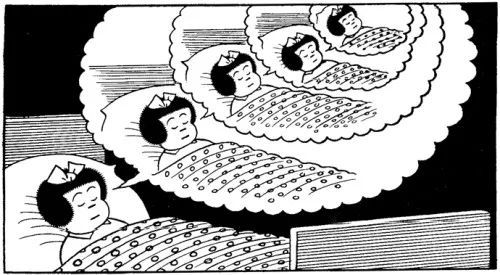
\includegraphics[scale=0.7]{img/Chapter5/5-3/1.png}
\end{figure}

\vspace{0.5cm}

\mybox{讲故事}

\begin{lstlisting}[language=C++]
#include <iostream>
#include <string>

using namespace std;

void tell_story() {
	string story;
	story += "从前有座山,山里有座庙\n";
	story += "庙里有个老和尚\n";
	story += "老和尚在对小和尚讲故事:\n";
	cout << story;

	tell_story();
}

int main() {
	tell_story();
	return 0;
}
\end{lstlisting}

\begin{tcolorbox}
	\mybox{运行结果}
	\begin{verbatim}
从前有座山,山里有座庙
庙里有个老和尚
老和尚在对小和尚讲故事:
从前有座山,山里有座庙
庙里有个老和尚
老和尚在对小和尚讲故事:
从前有座山,山里有座庙
庙里有个老和尚
老和尚在对小和尚讲故事:
...
	\end{verbatim}
\end{tcolorbox}

一个永远无法结束的递归函数最终会导致栈溢出。因此递归函数需要确定一个结束条件,确保在递归过程中能在合适的地方停止并返回。\\

\mybox{阶乘}

\begin{lstlisting}[language=C++]
#include <iostream>

using namespace std;

int factorial(int n) {
	if(n == 0 || n == 1) {
		return 1;
	}
	return n * factorial(n-1);
}

int main() {
	cout << "5! = " << factorial(5) << endl;
	return 0;
}
\end{lstlisting}

\begin{tcolorbox}
	\mybox{运行结果}
	\begin{verbatim}
5! = 120
	\end{verbatim}
\end{tcolorbox}

\begin{figure}[H]
	\centering
	\begin{tikzpicture}[]
		\draw (0,0) rectangle (3,1.5);
		\draw (3,-2) rectangle (6,-0.5);
		\draw (6,-4) rectangle (9,-2.5);
		\draw (9,-6) rectangle (12,-4.5);
		\draw (12,-8) rectangle (15,-6.5);

		\draw (12.75,-10.75) rectangle (14.25,-9.25);
		\draw (9.75,-8.75) rectangle (11.25,-7.25);
		\draw (6.75,-6.75) rectangle (8.25,-5.25);
		\draw (3.75,-4.75) rectangle (5.25,-3.25);
		\draw (0.75,-2.75) rectangle (2.25,-1.25);

		\draw (1.5,0.75) node {$ factorial(5) $};
		\draw (4.5,-1.25) node {$ factorial(4) $};
		\draw (7.5,-3.25) node {$ factorial(3) $};
		\draw (10.5,-5.25) node {$ factorial(2) $};
		\draw (13.5,-7.25) node {$ factorial(1) $};

		\draw (13.5,-10) node {$ 1 $};
		\draw (10.5,-8) node {$ 2 $};
		\draw (7.5,-6) node {$ 6 $};
		\draw (4.5,-4) node {$ 24 $};
		\draw (1.5,-2) node {$ 120 $};

		\draw[->] (3,0.75) -- (4.5,0.75) -- (4.5,-0.5);
		\draw[->] (6,-1.25) -- (7.5,-1.25) -- (7.5,-2.5);
		\draw[->] (9,-3.25) -- (10.5,-3.25) -- (10.5,-4.5);
		\draw[->] (12,-5.25) -- (13.5,-5.25) -- (13.5,-6.5);

		\draw[->] (12.75,-10) -- (10.5,-10) -- (10.5,-8.75);
		\draw[->] (9.75,-8) -- (7.5,-8) -- (7.5,-6.75);
		\draw[->] (6.75,-6) -- (4.5,-6) -- (4.5,-4.75);
		\draw[->] (3.75,-4) -- (1.5,-4) -- (1.5,-2.75);

		\draw (4.5,1) node {$ 5 * factorial(4) $};
		\draw (7.5,-1) node {$ 4 * factorial(3) $};
		\draw (10.5,-3) node {$ 3 * factorial(2) $};
		\draw (13.5,-5) node {$ 2 * factorial(1) $};

		\draw (11,-10.5) node {$ 2 * 1 $};
		\draw (8,-8.5) node {$ 3 * 2 $};
		\draw (5,-6.5) node {$ 4 * 6 $};
		\draw (2,-4.5) node {$ 5 * 24 $};
	\end{tikzpicture}
	\caption{阶乘}
\end{figure}

\vspace{0.5cm}

\mybox{斐波那契数列}

\begin{lstlisting}[language=C++]
#include <iostream>

using namespace std;

int fibonacci(int n) {
	if (n == 1 || n == 2) {
		return n;
	}
	return fibonacci(n - 2) + fibonacci(n - 1);
}

int main() {
	int n = 7;
	cout << fibonacci(n) << endl;
	return 0;
}
\end{lstlisting}

\begin{tcolorbox}
	\mybox{运行结果}
	\begin{verbatim}
21
	\end{verbatim}
\end{tcolorbox}

\begin{figure}[H]
	\centering
	\begin{tikzpicture}[
			level distance=2.4cm,
			level 1/.style={sibling distance=6cm},
			level 2/.style={sibling distance=3cm},
			level 3/.style={sibling distance=2cm}
		]
		\node {$ f(5) $}
		child {
				node {$ f(3) $}
				child {node {$ f(1) $}}
				child {node {$ f(2) $}}
			}
		child {
				node {$ f(4) $}
				child {node {$ f(2) $}}
				child {
						node {$ f(3) $}
						child {node {$ f(1) $}}
						child {node {$ f(2) $}}
					}
			};
	\end{tikzpicture}
	\caption{递归树}
\end{figure}

递归的特点就是将一个复杂的大问题逐步简化为一个可以解决的小问题,然后再逐步计算出大问题的解。\\

递归的优点在于代码简洁易懂,但是缺点也很明显,就是效率很低。每次递归都会产生函数调用,而函数调用的开销是很大的,不适合用来解决大规模的问题。\\

例如在计算斐波那契数列的第40项时,递归需要花费大量时间,因为其中包含了大量的重复计算。相比而言,使用循环的方式能够节省大量的时间。因此像阶乘和斐波那契数列这样的情况,通常会采用循环,而不是递归进行计算。\\

然而还存在很多问题不得不使用递归的思想才能解决。\\

\mybox{阿克曼函数}

\begin{align}\nonumber
	A(m, n) =
	\begin{cases}
		n + 1             & m = 0        \\
		A(m-1, 1)         & m > 0, n = 0 \\
		A(m-1, A(m, n-1)) & m > 0, n > 0 \\
	\end{cases}
\end{align}

\begin{lstlisting}[language=C++]
#include <iostream>

using namespace std;

int A(int m, int n) {
	if (m == 0) {
		return n + 1;
	} else if (m > 0 && n == 0) {
		return A(m - 1, 1);
	} else {
		return A(m - 1, A(m, n - 1));
	}
}

int main() {
	cout << A(3, 4) << endl;
	return 0;
}
\end{lstlisting}

\begin{tcolorbox}
	\mybox{运行结果}
	\begin{verbatim}
125
	\end{verbatim}
\end{tcolorbox}

\vspace{0.5cm}

\mybox{汉诺塔}\\

有三根柱子A、B、C,A柱子上从下到上套有n个圆盘,要求将A柱子上的圆盘移动到C柱子上。每次只能移动一个圆盘,且大圆盘始终不能叠在小圆盘上面。\\

\begin{figure}[H]
	\centering
	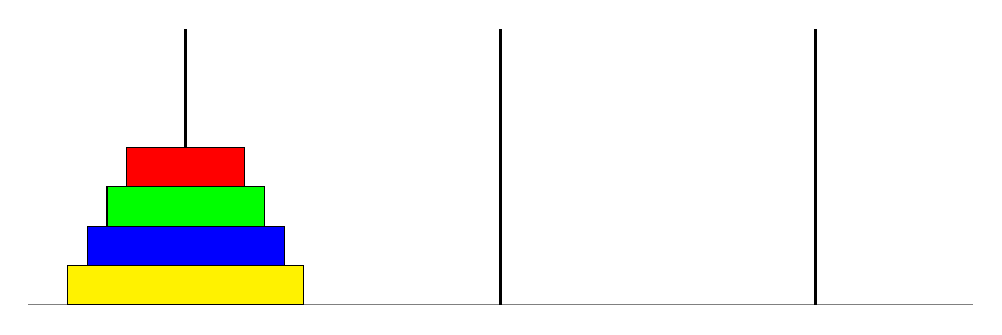
\begin{tikzpicture}[scale=0.5]
		\draw[-, gray] (0,0) -- (24,0);
		\draw[-, very thick] (4,0) -- (4,7);
		\draw[-, very thick] (12,0) -- (12,7);
		\draw[-, very thick] (20,0) -- (20,7);

		\draw[fill=red] (2.5,3) rectangle (5.5,4);
		\draw[fill=green] (2,2) rectangle (6,3);
		\draw[fill=blue] (1.5,1) rectangle (6.5,2);
		\draw[fill=yellow] (1,0) rectangle (7,1);
	\end{tikzpicture}
	\caption{汉诺塔}
\end{figure}

递归算法求解汉诺塔问题:

\begin{enumerate}
	\item 将n-1个圆盘从A借助C移到B。
	\item 将第n个圆盘从A移到C。
	\item 将n-1个圆盘从B借助A移到C。
\end{enumerate}

\vspace{-0.5cm}

\begin{lstlisting}[language=C++]
#include <iostream>

using namespace std;

int moves = 0;

void hanoi(int n, char src, char mid, char dst) {
	if (n == 1) {
		cout << src << " -> " << dst << endl;
		moves++;
	} else {
		// move top n-1 disks from src to mid
		hanoi(n - 1, src, dst, mid);
		cout << src << " -> " << dst << endl;
		moves++;
		// move top n-1 disks from mid to dst
		hanoi(n - 1, mid, src, dst);
	}
}

int main() {
	hanoi(3, 'A', 'B', 'C');
	cout << "Moves: " << moves << endl;
	return 0;
}
\end{lstlisting}

\begin{tcolorbox}
	\mybox{运行结果}
	\begin{verbatim}
A -> C
A -> B
C -> B
A -> C
B -> A
B -> C
A -> C
Moves: 7
	\end{verbatim}
\end{tcolorbox}

假设每次移动花费1秒,解决一个64层的汉诺塔问题大约需要5800亿年。\\

\begin{figure}[H]
	\centering
	
\includegraphics[]{img/Chapter5/5-3/2.png}
\end{figure}

\newpage
\chapter{预处理}

\section{预处理}

\subsection{宏(Macro)}

宏是一种简单的文本替换工具,可以用于定义一个特定的常量或表达式,一般用大写表示。宏定义使用\#define指令,在编译期间,编译器会将程序中所有的宏替换为其内容。\\

与变量的定义不同的是,宏没有类型,也不占内存空间。\\

\mybox{圆}

\begin{lstlisting}[language=C++]
#include <iostream>
#define PI 3.14159

using namespace std;

double perimeter(double r) {
    return 2 * PI * r;
}

double area(double r) {
    return PI * r * r;
}

int main() {
    double radius;
    cout << "Enter radius: ";
    cin >> radius;

    cout << "Perimeter: " << perimeter(radius) << endl;
    cout << "Area: " << area(radius) << endl;

    return 0;
}
\end{lstlisting}

\begin{tcolorbox}
    \mybox{运行结果}
    \begin{verbatim}
Enter radius: 5
Perimeter: 31.42
Area: 78.54
	\end{verbatim}
\end{tcolorbox}

宏也可以像函数一样传递参数,但是宏的参数不会进行类型检查,宏最终同样也会在编译期间被展开。\\

但是由于宏定义的内容在编译时会被替换到代码中,有时候会导致运算的优先级发生改变。

\vspace{-0.5cm}

\begin{lstlisting}[language=C++]
#define SQUARE x * x
\end{lstlisting}

例如SQUARE(2 + 3)会被展开为2 + 3 * 2 + 3,而不是(2 + 3) * (2 + 3)。因此,最好在宏中使用括号来避免这种情况。

\vspace{-0.5cm}

\begin{lstlisting}[language=C++]
#define SQUARE (x * x)
\end{lstlisting}

\vspace{0.5cm}

\subsection{条件编译}

条件编译是一种在编译时根据宏的定义来决定是否编译某段代码的方法。\\

\mybox{斐波那契数列}

\begin{lstlisting}[language=C++]
#include <iostream>

using namespace std;

#define RECURSION

#ifdef RECURSION
int fibonacci(int n) {
    if (n == 0) {
        return 0;
    } else if (n == 1) {
        return 1;
    }
    return fibonacci(n - 1) + fibonacci(n - 2);
}
#else
int fibonacci(int n) {
    int seq[n];
    seq[0] = 0;
    seq[1] = 1;

    for (int i = 2; i <= n; i++) {
        seq[i] = seq[i - 1] + seq[i - 2];
    }

    return seq[n];
}
#endif

int main() {
    int n;
    cout << "Enter n: ";
    cin >> n;
    cout << fibonacci(n) << endl;
    return 0;
}
\end{lstlisting}

\begin{tcolorbox}
    \mybox{运行结果}
    \begin{verbatim}
Enter n: 7
13
	\end{verbatim}
\end{tcolorbox}

\newpage

\section{多文件编译}

\subsection{编译(Compile)}

集成开发环境IDE(Integrated Development Environment)包含了文本编辑器、编译器、调试器和其它工具,可以很方便地进行开发。但是对于大型项目,使用命令行编译更加灵活和高效。\\

\mybox{交换}

\begin{lstlisting}[language=C++]
#include <iostream>

using namespace std;

#define SWAP(a, b) {int t; t = a; a = b; b = t;}

int main() {
    int a = 1;
    int b = 2;

    cout << "Before: a = " << a << ", b = " << b << endl;
    SWAP(a, b);
    cout << "After: a = " << a << ", b = " << b << endl;

    return 0;
}
\end{lstlisting}

\vspace{-0.5cm}

\begin{lstlisting}
g++ -Wall swap.cpp -o swap
./swap
\end{lstlisting}

其中g++表示编译器的名称,-Wall表示要输出所有警告信息,swap.cpp为需编译的源文件,-o用于指定输出的可执行文件的名称为swap。编译成功后使用./swap即可运行。\\

一个完整的编译过程包含4个步骤:

\begin{enumerate}
    \item 预处理:将头文件、宏定义等展开
          \vspace{-0.5cm}
          \begin{lstlisting}
g++ -E swap.cpp -o swap.i
            \end{lstlisting}

    \item 编译:将预处理后的代码转换为汇编代码
          \vspace{-0.5cm}
          \begin{lstlisting}
g++ -S swap.i -o swap.s
            \end{lstlisting}

    \item 汇编:将汇编代码转换为机器码
          \vspace{-0.5cm}
          \begin{lstlisting}
g++ -c swap.s -o swap.o
            \end{lstlisting}

    \item 链接:将目标文件链接为可执行文件
          \vspace{-0.5cm}
          \begin{lstlisting}
g++ swap.o -o swap
            \end{lstlisting}
\end{enumerate}

\vspace{0.5cm}

\subsection{多文件编译}

模块化编程的目的是为了将程序分解成多个独立、可重用的部分。当程序变得复杂时,分成多个文件可以使得程序逻辑更加清晰、易于维护。\\

在多文件中,每个模板一般都分为.h和.cpp两部分,其中.h文件用于声明函数原型,.cpp文件用于实现函数。这样其它文件只需要包含.h文件即可使用这些函数,就像包含头文件iostream一样,只不过自定义的头文件一般使用双引号包含。\\

由于一个头文件可以被多个源文件包含,为了避免重复定义,一般在头文件的开头使用条件编译来判断是否已经被包含。\\

\mybox{面积}

\begin{lstlisting}[language=C, title=geometry.h]
#ifndef _GEOMETRY_H_
#define _GEOMETRY_H_

double circle_area(double radius);

double triangle_area(double base, double height);

#endif
\end{lstlisting}

\begin{lstlisting}[language=C, title=geometry.c]
#include "geometry.h"

#define PI 3.1415926

double circle_area(double radius) {
    return PI * radius * radius;
}

double triangle_area(double base, double height) {
    return base * height / 2;
}
\end{lstlisting}

\begin{lstlisting}[language=C, title=area.c]
#include <stdio.h>
#include "geometry.h"

int main() {
    printf("Area of circle: %.2f\n", circle_area(5));
    printf("Area of triangle: %.2f\n", triangle_area(5, 10));
    return 0;
}
\end{lstlisting}

\vspace{-0.5cm}

\begin{lstlisting}
gcc -Wall geometry.c area.c -o area
./area
\end{lstlisting}

\begin{tcolorbox}
    \mybox{运行结果}
    \begin{verbatim}
Area of circle: 78.54
Area of triangle: 25.00
	\end{verbatim}
\end{tcolorbox}

\newpage
\chapter{指针}

\section{指针}

\subsection{指针(Pointer)}

每个变量都会在内存中占用一定的空间,不同类型的变量占用的空间大小也不同。每个空间都有一个地址,一般采用十六进制表示,如0x0060FEFC。\\

有时候需要通过变量的地址对变量进行操作,这时候就需要将变量的地址保存起来,保存地址的变量就成为指针。

\begin{figure}[H]
    \centering
    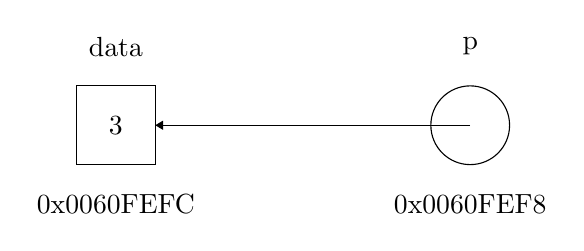
\begin{tikzpicture}
        \draw (0,0) rectangle node{3} (1,1);
        \draw (0.5,1.5) node{data};
        \draw (0.5,-0.5) node{0x0060FEFC};

        \draw (5,0.5) circle (0.5);
        \draw (5,1.5) node{p};
        \draw (5,-0.5) node{0x0060FEF8};

        \draw[->] (5,0.5) -- (1,0.5);
    \end{tikzpicture}
\end{figure}

*用于声明一个指针变量,例如int *p表示p是一个指针,指向一个int类型的变量的地址。通过取地址运算符\&可以获取变量的地址,占位符\%p能够以十六进制的形式输出地址。\\

既然指针保存了另一个变量的地址,那么通过指针就可以访问到那个变量上的数据。在指针变量前使用*运算符,就可以获取到指针所指向的变量的值。

\begin{figure}[H]
    \centering
    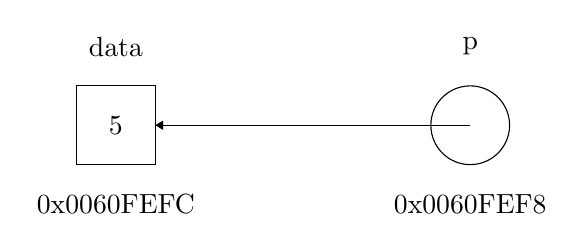
\begin{tikzpicture}
        \draw (0,0) rectangle node{5} (1,1);
        \draw (0.5,1.5) node{data};
        \draw (0.5,-0.5) node{0x0060FEFC};

        \draw (5,0.5) circle (0.5);
        \draw (5,1.5) node{p};
        \draw (5,-0.5) node{0x0060FEF8};

        \draw[->] (5,0.5) -- (1,0.5);
    \end{tikzpicture}
\end{figure}

\mybox{指针}

\begin{lstlisting}[language=C++]
#include <iostream>

using namespace std;

int main() {
    int data = 3;
    int *p = &data;

    cout << "Value of data: " << data << endl;
    cout << "Address of data: " << &data << endl;

    cout << "Value of p: " << p << endl;
    cout << "Address of p: " << &p << endl;
    cout << "Value of data pointed by p: " << *p << endl;
    
    *p = 5;

    cout << "Value of data: " << data << endl;
    cout << "Value of data pointed by p: " << *p << endl;

    return 0;
}
\end{lstlisting}

\begin{tcolorbox}
    \mybox{运行结果}
    \begin{verbatim}
Value of data: 3
Address of data: 0x61fe1c
Value of p: 0x61fe1c
Address of p: 0x61fe10
Value of data pointed by p: 3
Value of data: 5
Value of data pointed by p: 5
	\end{verbatim}
\end{tcolorbox}

为什么不直接修改变量的值,还要多此一举通过指针修改呢?\\

例如需要实现swap()用于交换两个变量的值,由于传递参数是按值传递(pass by value),所以交换的仅仅只是swap()中局部变量的值。\\

这种情况下就需要使用指针,将需要交换的变量的地址传递给swap(),然后在swap()中交换这两个地址上的值。\\

\mybox{交换}

\begin{lstlisting}[language=C++]
#include <iostream>

using namespace std;

void swap(int *data1, int *data2) {
    int temp = *data1;
    *data1 = *data2;
    *data2 = temp;
}

int main() {
    int a = 3;
    int b = 5;

    cout << "Before: a = " << a << ", b = " << b << endl;
    swap(&a, &b);
    cout << "After: a = " << a << ", b = " << b << endl;
    return 0;
}
\end{lstlisting}

\begin{tcolorbox}
    \mybox{运行结果}
    \begin{verbatim}
Before: a = 3, b = 5
After: a = 5, b = 3
	\end{verbatim}
\end{tcolorbox}

函数最多只能返回一个值,但如果需要有多个值需要返回,就可以使用指针将数据带回。\\

\mybox{一元二次方程}

\begin{lstlisting}[language=C++]
#include <iostream>
#include <cmath>
#include <iomanip>

using namespace std;

/**
 * Solve quadratic equation ax^2 + bx + c = 0.
 * @param a coefficient of x^2
 * @param b coefficient of x
 * @param c constant
 * @param x1 pointer to the first root
 * @param x2 pointer to the second root
 * @return true if the equation has real roots, false otherwise.
 */
bool solver(double a, double b, double c, double *x1, double *x2) {
    double delta = b * b - 4 * a * c;
    if (delta < 0) {
        return false;
    }
    *x1 = (-b + sqrt(delta)) / (2 * a);
    *x2 = (-b - sqrt(delta)) / (2 * a);
    return true;
}

int main() {
    double a, b, c;
    double x1, x2;

    cout << "Quadratic equation ax^2 + bx + c = 0" << endl;
    cout << "Enter coefficients a, b, c: ";
    cin >> a >> b >> c;

    if (solver(a, b, c, &x1, &x2)) {
        cout << fixed << setprecision(2) 
             << "x1 = "  << x1 << ", x2 = " << x2 << endl;
    } else {
        cout << "No real roots" << endl;
    }

    return 0;
}
\end{lstlisting}

\begin{tcolorbox}
    \mybox{运行结果}
    \begin{verbatim}
Quadratic equation ax^2 + bx + c = 0
Enter coefficients a, b, c: 1 -9 20
x1 = 5.00, x2 = 4.00
	\end{verbatim}
\end{tcolorbox}

\vspace{0.5cm}

\subsection{NULL}

如果一个变量声明时没有初始化,那么它的值是不确定的。声明指针时如果不对指针进行初始化,那么它就会指向一块不确定的内存地址,这种指针被称为野指针。\\

使用野指针可能会导致程序崩溃,因为它可能指向一个不可访问的内存地址。因此,如果指针没有指向一个确定的内存地址时,应该将其赋值为空指针NULL。

\vspace{-0.5cm}

\begin{lstlisting}[language=C++]
int *p = NULL;
\end{lstlisting}

\newpage

\section{指针与数组}

\subsection{指针与数组}

数组名本质上就是一个指针,它指向数组的首地址。因此在获取数组的地址时,可以不使用\&运算符。\\

\begin{figure}[H]
    \centering
    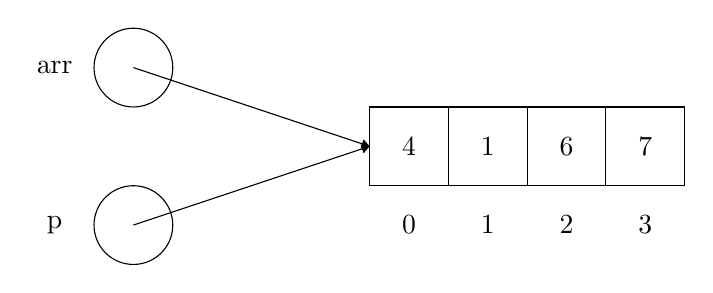
\begin{tikzpicture}
        \draw (0,1) circle (0.5);
        \draw (-1,1) node{arr};

        \draw (0,-1) circle (0.5);
        \draw (-1,-1) node{p};

        \draw (3,-0.5) rectangle (7,0.5);
        \draw (4,-0.5) -- (4,0.5);
        \draw (5,-0.5) -- (5,0.5);
        \draw (6,-0.5) -- (6,0.5);

        \draw (3.5,0) node {4};
        \draw (4.5,0) node {1};
        \draw (5.5,0) node {6};
        \draw (6.5,0) node {7};

        \draw (3.5,-1) node {0};
        \draw (4.5,-1) node {1};
        \draw (5.5,-1) node {2};
        \draw (6.5,-1) node {3};

        \draw[->] (0,1) -- (3,0);
        \draw[->] (0,-1) -- (3,0);
    \end{tikzpicture}
\end{figure}

当对一个指向数组的指针进行加减运算时(如p++和p--),并不是将地址加1或减1,而是根据指针的类型加或减对应字节的长度。例如p是一个int型指针,那么p++会将地址加4(int占4个字节)、p -= 2会将地址减8。\\

\mybox{指针与数组}

\begin{lstlisting}[language=C++]
#include <iostream>

using namespace std;

int main() {
    int arr[] = {4, 1, 6, 7};
    int n = sizeof(arr) / sizeof(arr[0]);
    int *p = arr;

    cout << "Address of arr: " << arr << endl;
    for (int i = 0; i < n; i++) {
        cout << "Address of arr[" << i << "]: " << &arr[i] << endl;
    }

    cout << "Value of p: " << p << endl;
    for (int i = 1; i < n; i++) {
        cout << "Value of p + " << i << ": " << p + i << endl;
    }

    *p = 9;
    *(p + 1) = 8;
    *(p + 2) = 7;
    *(p + 3) = 6;

    for (int i = 0; i < n; i++) {
        cout << "arr[" << i << "]: " << arr[i] << endl;
    }

    return 0;
}
\end{lstlisting}

\begin{tcolorbox}
    \mybox{运行结果}
    \begin{verbatim}
Address of arr: 0x61fdf0   
Address of arr[0]: 0x61fdf0
Address of arr[1]: 0x61fdf4
Address of arr[2]: 0x61fdf8
Address of arr[3]: 0x61fdfc
Value of p: 0x61fdf0
Value of p + 1: 0x61fdf4
Value of p + 2: 0x61fdf8
Value of p + 3: 0x61fdfc
arr[0]: 9
arr[1]: 8
arr[2]: 7
arr[3]: 6
	\end{verbatim}
\end{tcolorbox}

\vspace{0.5cm}

\subsection{数组与函数}

数组作为函数参数时,会将数组的地址传递给函数,函数接收到的是一个指向数组首地址的指针。由于在函数中失去了数组长度的信息,并不能通过sizeof()计算出数组的长度(计算得到的是一个指针变量所占的空间),因此将数组传入函数时,还需要将其长度一并作为参数传给函数。\\

\mybox{查找}

\begin{lstlisting}[language=C++]
#include <iostream>

using namespace std;

int search(int *arr, int n, int key) {
    for (int i = 0; i < n; i++) {
        if (arr[i] == key) {
            return i;
        }
    }
    return -1;
}

int main() {
    int arr[] = {4, 7, 1, 3, 9, 2};
    int n = sizeof(arr) / sizeof(arr[0]);

    int index = search(arr, n, 3);
    if (index == -1) {
        cout << "Not found" << endl;
    } else {
        cout << "Found at index " << index << endl;
    }

    return 0;
}
\end{lstlisting}

\begin{tcolorbox}
    \mybox{运行结果}
    \begin{verbatim}
Found at index 3
	\end{verbatim}
\end{tcolorbox}

\newpage

\section{指针与字符串}

\subsection{指针与字符串}

数组和指针都可以用于定义一个字符串,但是它们内存分配的方式不同,从而导致它们的使用方式也不同。\\

以数组形式定义的字符串,每个字符保存在一个字符数组中。这样的字符串是可以修改的,与普通的数组类似。\\

但是如果让一个指针指向一个字符串,那么这个字符串会被存储在常量区。常量区中的数据是不可以修改的,因此使用指针去修改字符串会导致程序崩溃。\\

\begin{figure}[H]
    \centering
    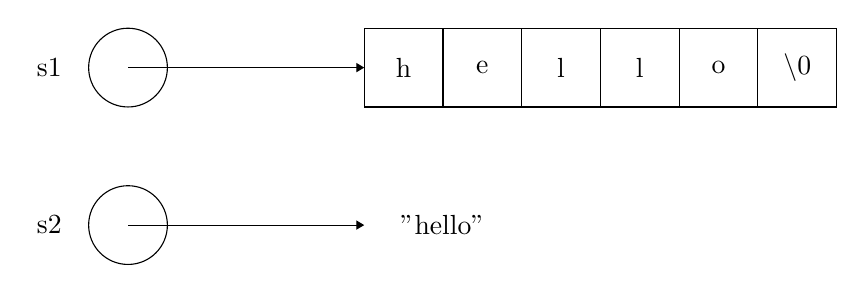
\begin{tikzpicture}
        \draw (0,0) circle (0.5);
        \draw (-1,0) node{s1};

        \draw (3,-0.5) rectangle (9,0.5);
        \draw (4,-0.5) -- (4,0.5);
        \draw (5,-0.5) -- (5,0.5);
        \draw (6,-0.5) -- (6,0.5);
        \draw (7,-0.5) -- (7,0.5);
        \draw (8,-0.5) -- (8,0.5);

        \draw (3.5,0) node {h};
        \draw (4.5,0) node {e};
        \draw (5.5,0) node {l};
        \draw (6.5,0) node {l};
        \draw (7.5,0) node {o};
        \draw (8.5,0) node {$ \backslash $0};

        \draw[->] (0,0) -- (3,0);

        \draw (0,-2) circle (0.5);
        \draw (-1,-2) node{s2};
        \draw (4,-2) node {"hello"};
        \draw[->] (0,-2) -- (3,-2);
    \end{tikzpicture}
\end{figure}

\vspace{-0.5cm}

\begin{lstlisting}[language=C++]
char s1[] = "hello";
s1[0] = 'H';
cout << s1 << endl;

char *s2 = "hello";
s2[0] = 'H';        // error
cout << s2 << endl;
\end{lstlisting}

在对指向字符串的指针进行赋值操作的时候,并不会产生新的字符串,只是让两个指针都指向同一个字符串,对任意一个指针做的操作都会影响另一个指针。\\

\begin{figure}[H]
    \centering
    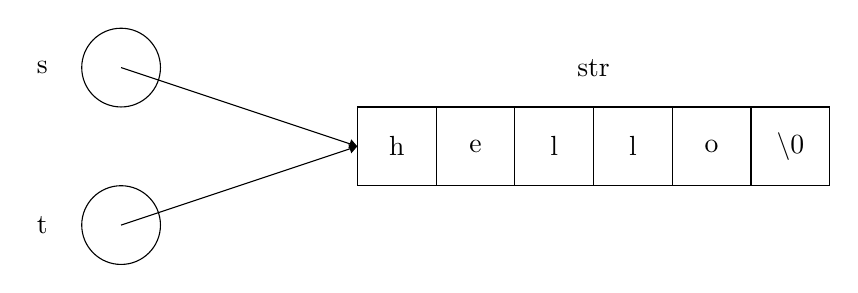
\begin{tikzpicture}
        \draw (0,1) circle (0.5);
        \draw (-1,1) node{s};

        \draw (0,-1) circle (0.5);
        \draw (-1,-1) node{t};

        \draw (3,-0.5) rectangle (9,0.5);
        \draw (4,-0.5) -- (4,0.5);
        \draw (5,-0.5) -- (5,0.5);
        \draw (6,-0.5) -- (6,0.5);
        \draw (7,-0.5) -- (7,0.5);
        \draw (8,-0.5) -- (8,0.5);

        \draw (3.5,0) node {h};
        \draw (4.5,0) node {e};
        \draw (5.5,0) node {l};
        \draw (6.5,0) node {l};
        \draw (7.5,0) node {o};
        \draw (8.5,0) node {$ \backslash $0};
        \draw (6,1) node {str};

        \draw[->] (0,1) -- (3,0);
        \draw[->] (0,-1) -- (3,0);
    \end{tikzpicture}
\end{figure}

\mybox{指向字符串的指针}

\begin{lstlisting}[language=C++]
#include <iostream>

using namespace std;

int main() {
    char str[] = "hello";
    char *s = str;
    char *t = s;

    s[0] = 'H';
    cout << "s = " << s << endl;
    cout << "t = " << t << endl;

    return 0;
}
\end{lstlisting}

\begin{tcolorbox}
    \mybox{运行结果}
    \begin{verbatim}
s = Hello
t = Hello
	\end{verbatim}
\end{tcolorbox}

\newpage

\section{二级指针}

\subsection{二级指针(Pointer to pointer)}

既然指针也是一个变量,那么一个指针也可以指向另一个指针,这样的指针称为二级指针。

\begin{figure}[H]
    \centering
    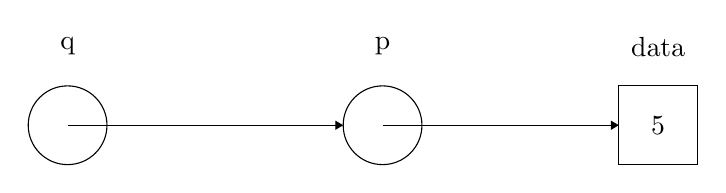
\begin{tikzpicture}
        \draw (0,0) circle (0.5);
        \draw (0,1) node{q};
        \draw (4,0) circle (0.5);
        \draw (4,1) node{p};

        \draw (7,-0.5) rectangle (8,0.5);
        \draw (7.5,0) node {5};
        \draw (7.5,1) node {data};

        \draw[->] (0,0) -- (3.5,0);
        \draw[->] (4,0) -- (7,0);
    \end{tikzpicture}
\end{figure}

其中p是一个int型的指针(int *),指向了data;q是一个指向int型指针的指针(int **),即q指向了一个指向int的指针。\\

\mybox{二级指针}

\begin{lstlisting}[language=C++]
#include <iostream>

using namespace std;

int main() {
    int data = 5;
    int *p = &data;
    int **q = &p;

    cout << "data = " << data << endl;
    cout << "*p = " << *p << endl;
    cout << "**q = " << **q << endl;

    cout << "Address of data = " << &data << endl;
    cout << "Address of p = " << &p << endl;
    cout << "Address of q = " << &q << endl;

    cout << "Value of p = " << p << endl;
    cout << "Value of q = " << q << endl;

    return 0;
}
\end{lstlisting}

\begin{tcolorbox}
    \mybox{运行结果}
    \begin{verbatim}
data = 5
*p = 5  
**q = 5
Address of data = 0x61fe1c
Address of p = 0x61fe10
Address of q = 0x61fe08
Value of p = 0x61fe1c
Value of q = 0x61fe10
	\end{verbatim}
\end{tcolorbox}

\vspace{0.5cm}

\subsection{指针与二维数组}

二级指针还可以用于表示二维数组。与一维数组类似,可以使用下标或*运算符来访问二维数组中的元素。\\

\begin{figure}[H]
    \centering
    \begin{tikzpicture}
        \draw (0,1.5) circle (0.5);
        \draw (0,2.5) node{arr};
        \draw (4,1.5) circle (0.5);

        \draw (7,-2) rectangle (11,2);
        \draw (8,-2) -- (8,2);
        \draw (9,-2) -- (9,2);
        \draw (10,-2) -- (10,2);
        \draw (7,-1) -- (11,-1);
        \draw (7,0) -- (11,0);
        \draw (7,1) -- (11,1);

        \draw[->] (0,1.5) -- (3.5,1.5);
        \draw[->] (4,1.5) -- (7,1.5);
    \end{tikzpicture}
\end{figure}

例如,arr[2][1]也可以写成*(*(arr + 2) + 1)。

\begin{figure}[H]
    \centering
    \begin{tikzpicture}
        \draw (0,1.5) circle (0.5);
        \draw (0,2.5) node{arr};
        \draw (4,1.5) circle (0.5);

        \draw (7,-2) rectangle (11,2);
        \draw (8,-2) -- (8,2);
        \draw (9,-2) -- (9,2);
        \draw (10,-2) -- (10,2);
        \draw (7,-1) -- (11,-1);
        \draw (7,0) -- (11,0);
        \draw (7,1) -- (11,1);

        \draw[->] (0,1.5) -- (3.5,1.5);
        \draw[->] (4,1.5) -- (8.5,-0.5);
    \end{tikzpicture}
\end{figure}

当如果命令行运行时,可以向main()函数传递命令行参数。传递参数的数量和值可以通过argc(argument count)和argv(argument vector)来获取。argv为一个二维数组,每个元素都是一个字符串,其中argv[0]为当前程序的名称。\\

\mybox{命令行参数}

\begin{lstlisting}[language=C++]
#include <iostream>
#include <cctype>
#include <cstring>

using namespace std;

char *lower(char *s) {
    char *p = s;
    while (*p) {
        *p = tolower(*p);
        p++;
    }
    return s;
}

char *upper(char *s) {
    char *p = s;
    while (*p) {
        *p = toupper(*p);
        p++;
    }
    return s;
}

void usage(const char *program) {
    cout << "Usage: " << program << " [option] [string]" << endl;
    cout << "--lower: convert string to lower case" << endl;
    cout << "--upper: convert string to upper case" << endl;
}

int main(int argc, char **argv) {
    if (argc != 3) {
        usage(argv[0]);
        return 1;
    }

    char *option = argv[1];
    char *string = argv[2];

    if (strcmp(option, "--lower") == 0) {
        cout << "Lower: " << lower(string) << endl;
    } else if (strcmp(option, "--upper") == 0) {
        cout << "Upper: " << upper(string) << endl;
    } else {
        usage(argv[0]);
        return 1;
    }

    return 0;
}
\end{lstlisting}

\begin{lstlisting}
g++ -Wall command_line.cpp -o command_line
./command_line --upper "Hello World!"
\end{lstlisting}

\begin{tcolorbox}
    \mybox{运行结果}
    \begin{verbatim}
Upper: HELLO WORLD!
	\end{verbatim}
\end{tcolorbox}

\newpage

\section{引用}

\subsection{引用(Reference)}

引用可以看作是变量的别名,对引用的操作与对变量的操作完全一样。因此引用可以用于传递参数和返回值,避免了复制较大变量的开销。\\

声明引用时必须对其初始化,并且之后不能再将该引用作为其它变量的别名。\\

\mybox{交换}

\begin{lstlisting}[language=C++]
#include <iostream>

using namespace std;

void swap(int &data1, int &data2) {
    int temp = data1;
    data1 = data2;
    data2 = temp;
}

int main() {
    int a = 3;
    int b = 5;

    cout << "Before: a = " << a << ", b = " << b << endl;
    swap(a, b);
    cout << "After: a = " << a << ", b = " << b << endl;
    return 0;
}
\end{lstlisting}

\begin{tcolorbox}
    \mybox{运行结果}
    \begin{verbatim}
Before: a = 3, b = 5
After: a = 5, b = 3
	\end{verbatim}
\end{tcolorbox}

\vspace{0.5cm}

\begin{table}[H]
    \centering
    \setlength{\tabcolsep}{5mm}{
        \begin{tabular}{|c|c|c|}
            \hline
                                  & \textbf{指针}         & \textbf{引用}    \\
            \hline
            \textbf{内存}         & 占用空间              & 不占用空间       \\
            \hline
            \textbf{大小}         & 4字节/8字节           & 被引用对象的大小 \\
            \hline
            \textbf{能否为空}     & 可以为NULL            & 引用对象必须存在 \\
            \hline
            \textbf{能否改变指向} & 可以                  & 不可以           \\
            \hline
            \textbf{使用}         & 通过*对指向的变量操作 & 直接对变量操作   \\
            \hline
            \textbf{层级}         & 可以有多级指针        & 只有一级         \\
            \hline
        \end{tabular}
    }
    \caption{指针与引用的区别}
\end{table}

\newpage

\section{动态内存申请}

\subsection{内存管理}

计算机的内存主要包括:

\begin{enumerate}
    \item 代码区:存储程序执行时使用的指令。
    \item 数据区:存储程序运行时使用的全局变量和静态变量。
    \item 栈区(stack):存储函数调用时使用的局部变量,栈中的内存由编译器自动分配和释放。
    \item 堆区(heap):存储动态分配内存的变量,需要由程序员自己分配和释放。
\end{enumerate}

\begin{figure}[H]
    \centering
    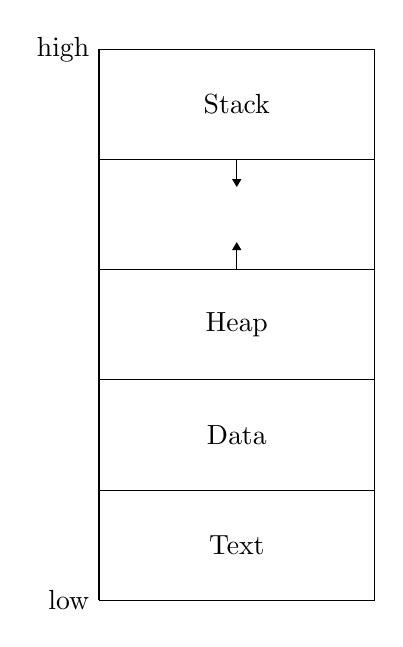
\begin{tikzpicture}[scale=0.7]
        \draw[-] (0,0) -- (0,10) -- (5,10) -- (5,0) -- (0,0);
        \draw[-] (0,2) -- (5,2);
        \draw[-] (0,4) -- (5,4);
        \draw[-] (0,6) -- (5,6);
        \draw[-] (0,8) -- (5,8);

        \draw (0,0) node[left] {low};
        \draw (0,10) node[left] {high};

        \draw (2.5,1) node {Text};
        \draw (2.5,3) node {Data};
        \draw (2.5,5) node {Heap};
        \draw (2.5,9) node {Stack};

        \draw[->] (2.5,8) -- (2.5,7.5);
        \draw[->] (2.5,6) -- (2.5,6.5);
    \end{tikzpicture}
    \caption{内存区域}
\end{figure}

有时候需要在函数中生成一个数组,并且将数组返回给调用者。但是在函数内定义的数组是局部变量,存储于栈区。函数执行完毕后,数组所占用的内存空间会被释放。因此被返回的数组的指针指向的是一个已经被释放的内存空间,这样就会导致程序崩溃。\\

另一种情况是,由于数组一旦声明后,其容量就不能再改变。当需要在运行时动态改变数组容量时,就可以采用动态内存申请的方式。\\

\subsection{malloc()}

malloc()函数定义在<cstdlib>中,用于在堆区申请一块内存空间,其函数原型为:

\vspace{-0.5cm}

\begin{lstlisting}[language=C++]
void* malloc(size_t size);
\end{lstlisting}

malloc()接受一个参数size,表示申请空间的大小(单位:字节),并返回指向申请到的空间的首地址的指针。如果申请失败,则返回NULL。\\

malloc()返回的是无类型指针void *,这是由于malloc()只负责申请指定大小的空间,并不关心这块空间将会被存放什么类型的数据。因此,开发者需要自行将其转换为对应的类型。\\

\mybox{内存}

\begin{lstlisting}[language=C++]
#include <iostream>
#include <cstdlib>

using namespace std;

int main() {
    void *p;
    int cnt = 0;

    // allocate 100MB memory each time
    while ((p = malloc(100 * 1024 * 1024))) {
        cnt++;
    }
    cout << "Allocated " << cnt * 100 << " MB memory" << endl;

    return 0;
}
\end{lstlisting}

\begin{tcolorbox}
    \mybox{运行结果}
    \begin{verbatim}
Allocated 57700 MB memory
	\end{verbatim}
\end{tcolorbox}

\vspace{0.5cm}

\subsection{free()}

通过动态申请来的内存空间需要是需要归还给操作系统,因此需要程序员自行在不需要使用时将其释放。如果不释放内存,这些动态申请的内存空间就会一直占用着,直到程序结束统一被操作系统释放。\\

不释放内存会导致内存泄漏(memory leak),如果一直分配内存而不是释放,最终将会耗尽所有可用的内存,导致程序运行变慢或者崩溃。\\

free()函数用于释放动态申请的内存空间,其接受一个参数ptr,表示要释放的内存空间的首地址。其函数原型为:

\vspace{-0.5cm}

\begin{lstlisting}[language=C++]
void free(void *ptr);
\end{lstlisting}

\vspace{0.5cm}

\mybox{斐波那契数列}

\begin{lstlisting}[language=C++]
#include <iostream>
#include <cstdlib>

using namespace std;

int *generate_fibonacci(int n) {
    int *arr = (int *)malloc(n * sizeof(int));
    if (!arr) {
        return NULL;
    }

    arr[0] = 1;
    arr[1] = 1;
    for (int i = 2; i < n; i++) {
        arr[i] = arr[i - 1] + arr[i - 2];
    }
    return arr;
}

int main() {
    int n = 10;
    int *arr = generate_fibonacci(n);

    for (int i = 0; i < n; i++) {
        cout << arr[i] << " ";
    }
    cout << endl;

    free(arr);
    return 0;
}
\end{lstlisting}

\begin{tcolorbox}
    \mybox{运行结果}
    \begin{verbatim}
1 1 2 3 5 8 13 21 34 55
	\end{verbatim}
\end{tcolorbox}

\vspace{0.5cm}

\subsection{calloc()}

calloc()与malloc()功能类似,也是用于动态申请内存空间的。只是malloc()只接受一个参数作为申请空间的大小,申请到的空间并不会进行初始化;而calloc()接受两个参数,可以申请多个指定大小的空间,并将这些空间初始化为0。calloc()的函数原型为:

\vspace{-0.5cm}

\begin{lstlisting}[language=C++]
void *calloc(size_t nitems, size_t size);
\end{lstlisting}

例如需要申请一个长度为n的int数组,并将其初始化为0:

\vspace{-0.5cm}

\begin{lstlisting}[language=C++]
int *arr = (int *)calloc(n, sizeof(int));
\end{lstlisting}

\vspace{0.5cm}

\subsection{realloc()}

realloc()用于对已经动态申请的内存空间进行重新分配(扩容/缩小),其函数原型为:

\vspace{-0.5cm}

\begin{lstlisting}[language=C++]
void *realloc(void *ptr, size_t size);
\end{lstlisting}

realloc()接受两个参数,第一个参数ptr指向需要重新分配内存空间,第二个参数size表示重新分配空间的大小(单位:字节)。realloc()会将原来内存块中的数据复制到新分配的内存块中,并返回指向新内存块的指针。如果重新分配失败,则返回NULL。\\

\mybox{strip}

\begin{lstlisting}[language=C++]
#include <iostream>
#include <cstdlib>
#include <cstring>
#include <cctype>

using namespace std;

char *strip(char *str) {
    int i = 0;
    int j = strlen(str) - 1;

    while (isspace(str[i]) && str[i] != '\0') {
        i++;
    }

    while (isspace(str[j]) && j >= 0) {
        j--;
    }

    int k = 0;
    while (i <= j) {
        str[k++] = str[i++];
    }
    str[k] = '\0';

    str = (char *)realloc(str, (k + 1) * sizeof(char));
    return str;
}

int main() {
    int len = 32;
    char *str = (char *)calloc(len + 1, sizeof(char));

    strcpy(str, "     Hello World! \n\t ");
    cout << "Before: [" << str << "]" << endl;

    str = strip(str);

    cout << "After: [" << str << "]" << endl;

    free(str);
    return 0;
}
\end{lstlisting}

\begin{tcolorbox}
    \mybox{运行结果}
    \begin{verbatim}
Before: [     Hello World! 
     ]
After: [Hello World!]
	\end{verbatim}
\end{tcolorbox}

\newpage
\chapter{文件}

\section{文件}

\subsection{fopen()}

文件是存储数据的一种常用方式,程序可以从文件中读取和写入数据,从而实现对数据的持久化存储。\\

在对文件进行操作之前,首先需要使用fopen()函数打开文件,fopen()的函数原型为:

\vspace{-0.5cm}

\begin{lstlisting}[language=C++]
FILE *fopen(const char *filename, const char *mode);
\end{lstlisting}

fopen()接受两个参数,第一个参数是要打开的文件名,第二个参数为打开方式。fopen()会返回一个FILE类型的指针,通过该指针可以对文件进行操作;如果文件打开失败,则返回NULL。\\

\begin{table}[H]
    \centering
    \setlength{\tabcolsep}{5mm}{
        \begin{tabular}{|c|l|}
            \hline
            \textbf{打开方式} & \textbf{功能}                                      \\
            \hline
            r                 & 只读,文件必须存在,否则打开失败                   \\
            \hline
            w                 & 只写,创建一个新文件                               \\
            \hline
            a                 & 追加,如果文件不存在则创建;存在则将数据追加到末尾 \\
            \hline
            r+                & 以r模式打开文件,附带写的功能                      \\
            \hline
            w+                & 以w模式打开文件,附带读的功能                      \\
            \hline
            a+                & 以a模式打开文件,附带读的功能                      \\
            \hline
        \end{tabular}
    }
    \caption{文件打开方式}
\end{table}

\vspace{0.5cm}

\subsection{fclose()}

在对文件操作结束后,需要使用fclose()函数将文件关闭。fclose()函数原型:

\vspace{-0.5cm}

\begin{lstlisting}[language=C++]
int fclose(FILE *stream);
\end{lstlisting}

\vspace{0.5cm}

\mybox{文件}

\begin{lstlisting}[title=data.txt]
This is a test.
\end{lstlisting}

\begin{lstlisting}[language=C++]
#include <iostream>
#include <cstdlib>

using namespace std;

int main() {
    FILE *fp = fopen("data.txt", "r");
    if(!fp) {
        exit(1);
    }
    fclose(fp);
    return 0;
}
\end{lstlisting}

\newpage

\section{文件I/O}

\subsection{fprintf()}

fprintf()函数用于将数据输出到文件中,使用方法与printf()类似。fprintf()的函数原型为:

\vspace{-0.5cm}

\begin{lstlisting}[language=C++]
int fprintf(FILE *stream, const char *format, ...);
\end{lstlisting}

\vspace{0.5cm}

\mybox{成绩}

\begin{lstlisting}[language=C++]
#include <iostream>
#include <cstdlib>

using namespace std;

int main() {
    FILE *fp = fopen("data1.txt", "w");
    int n;
    cout << "Enter number of students: ";
    cin >> n;

    char id[8];
    double score;
    for (int i = 0; i < n; i++) {
        cout << "Enter student " << i + 1 << "'s ID: ";
        cin >> id;
        cout << "Enter student " << i + 1 << "'s score: ";
        cin >> score;
        fprintf(fp, "ID=%s\tScore=%.2f\n", id, score);
    }

    fclose(fp);
    return 0;
}
\end{lstlisting}

\begin{tcolorbox}
    \mybox{运行结果}
    \begin{verbatim}
Enter number of students: 5
Enter student 1's ID: A001
Enter student 1's score: 92
Enter student 2's ID: A002
Enter student 2's score: 73
Enter student 3's ID: A003
Enter student 3's score: 89
Enter student 4's ID: A004
Enter student 4's score: 97
Enter student 5's ID: A005
Enter student 5's score: 65
	\end{verbatim}
\end{tcolorbox}

\begin{tcolorbox}
    \mybox{运行结果}
    \textbf{data1.txt}
    \begin{verbatim}
ID=A001	Score=92.00
ID=A002	Score=73.00
ID=A003	Score=89.00
ID=A004	Score=97.00
ID=A005	Score=65.00
	\end{verbatim}
\end{tcolorbox}

为了统一对各种硬件的操作,不同的硬件设备也都被看作是文件进行管理。计算机中标准输入(stdin)是键盘、标准输出(stdout)是显示器、标准错误(stderr)是显示器。\\

因此,当使用printf()函数时,其实是从将数据输出到显示器上。printf()函数是通过调用fprintf(stdout, ...)来实现的。\\

当需要输出一些错误信息时,可以通过fprintf(stderr, ...)将错误信息输出到标准错误stderr上,这样可以避免将错误信息混入到正常的输出信息中,方便查看和分析。\\

\subsection{fscanf()}

fscanf()函数用于从文件中读取数据,使用方法与scanf()类似。fscanf()的函数原型为:

\vspace{-0.5cm}

\begin{lstlisting}[language=C++]
int fscanf(FILE *stream, const char *format, ...);
\end{lstlisting}

fscanf()函数读取成功时返回实际读取的数据个数,失败时返回文件末尾标志EOF(End of File)。\\

\mybox{平均分}

\begin{lstlisting}[language=C++]
#include <iostream>
#include <cstdlib>
#include <iomanip>

using namespace std;

int main() {
    FILE *fp = fopen("data1.txt", "r");
    if (!fp) {
        cerr << "File open failed." << endl;
        exit(1);
    }

    char id[8];
    double score;
    double sum = 0;
    int n = 0;

    while (fscanf(fp, "ID=%s\tScore=%lf\n", id, &score) != EOF) {
        sum += score;
        n++;
    }
    cout << "Average = "
         << fixed << setprecision(2) << sum / n << endl;

    fclose(fp);
    return 0;
}
\end{lstlisting}

\begin{tcolorbox}
    \mybox{运行结果}
    \begin{verbatim}
Average = 83.20
	\end{verbatim}
\end{tcolorbox}

当使用scanf()函数时,其实是从键盘上读取数据的,scanf()函数是通过调用fscanf(stdin, ...)来实现的。\\

\subsection{fputc()}

fputc()函数用于将一个字符写入文件中,其函数原型为:

\vspace{-0.5cm}

\begin{lstlisting}[language=C++]
int fputc(int ch, FILE *stream);
\end{lstlisting}

fputc()接受两个参数,第一个参数为要写入的字符(ASCII码),第二个参数为文件指针。\\

当向屏幕输出一个字符时,fputc(stdout)等价于putchar()。\\

\mybox{大写字母}

\begin{lstlisting}[language=C++]
#include <iostream>
#include <cstdlib>

using namespace std;

int main() {
    FILE *fp = fopen("data2.txt", "w");

    for (int i = 0; i < 26; i++) {
        fputc('A' + i, fp);
    }

    fclose(fp);
    return 0;
}
\end{lstlisting}

\begin{tcolorbox}
    \mybox{运行结果}
    \textbf{data2.txt}
    \begin{verbatim}
ABCDEFGHIJKLMNOPQRSTUVWXYZ
	\end{verbatim}
\end{tcolorbox}

\vspace{0.5cm}

\subsection{fgetc()}

fgetc()函数用于从文件中读取一个字符,读取成功返回字符的ASCII码,失败返回EOF。fgetc()的函数原型为:

\vspace{-0.5cm}

\begin{lstlisting}[language=C++]
int fgetc(FILE *stream);
\end{lstlisting}

当从键盘读取一个字符时,fgetc(stdin)等价于getchar()。\\

在读取文件时,除了可以通过返回值EOF来判断是否读取到文件末尾外,还可以使用feof()函数,当读到文件末尾时返回非0值,否则返回0。feof()的函数原型为:

\vspace{-0.5cm}

\begin{lstlisting}[language=C++]
int feof(FILE *stream);
\end{lstlisting}

\vspace{0.5cm}

\mybox{源代码统计}

\begin{lstlisting}[language=C++]
#include <iostream>
#include <cstdlib>

using namespace std;

int main() {
    FILE *fp = fopen("statistics.cpp", "r");
    if (!fp) {
        cerr << "File open failed." << endl;
        exit(1);
    }

    int chars = 0;
    int lines = 0;

    while (!feof(fp)) {
        char c = fgetc(fp);
        if (c == '\n') {
            lines++;
        } else {
            chars++;
        }
    }

    cout << "Characters: " << chars << endl;
    cout << "Lines: " << lines << endl;

    fclose(fp);
    return 0;
}
\end{lstlisting}

\begin{tcolorbox}
    \mybox{运行结果}
    \begin{verbatim}
Characters: 485
Lines: 29
	\end{verbatim}
\end{tcolorbox}

\vspace{0.5cm}

\subsection{fputs()}

fputs()函数用于将一个字符串写入文件,其函数原型为:

\vspace{-0.5cm}

\begin{lstlisting}[language=C++]
int fputs(const char *str, FILE *stream);
\end{lstlisting}

当向屏幕输出一个字符串时,fputs(stdout)等价于puts()。\\

\mybox{Computer Science Quotes}

\begin{lstlisting}[language=C++]
#include <iostream>
#include <cstdlib>

using namespace std;

int main() {
    const char *quotes[] = {
        "Talk is cheap. Show me the code.",
        "Code never lies, comments sometimes do.",
        "Stay Hungry Stay Foolish.",
    };
    int n = sizeof(quotes) / sizeof(quotes[0]);

    FILE *fp = fopen("data3.txt", "w");

    for (int i = 0; i < n; i++) {
        fputs(quotes[i], fp);
        fputc('\n', fp);
    }

    fclose(fp);
    return 0;
}
\end{lstlisting}

\begin{tcolorbox}
    \mybox{运行结果}
    \textbf{data3.txt}
    \begin{verbatim}
Talk is cheap. Show me the code.
Code never lies, comments sometimes do.
Stay Hungry Stay Foolish.
	\end{verbatim}
\end{tcolorbox}

\vspace{0.5cm}

\subsection{fgets()}

fgets()函数用于从文件读取一行数据,读取成功返回指向字符串的指针,失败则返回NULL。fgets()的函数原型为:

\vspace{-0.5cm}

\begin{lstlisting}[language=C++]
char *fgets(char *str, int n, FILE *stream);
\end{lstlisting}

fgets()接受三个参数,第一个参数用于保存读取到的字符串,第二个参数用于指定读取的最大字符数(包括结尾的$ \backslash $0),第三个参数为文件指针。\\

\mybox{解析单词}

\begin{lstlisting}[language=C++]
#include <stdio.h>
#include <stdlib.h>
#include <string.h>
#include <ctype.h>

int main() {
    FILE *fp = fopen("data3.txt", "r");
    if (!fp) {
        fprintf(stderr, "File open failed.\n");
    }

    char line[128];
    while (fgets(line, sizeof(line), fp) != NULL) {
        char *token = strtok(line, " \t\n");
        while (token != NULL) {
            // remove punctuations
            int i = strlen(token) - 1;
            while (!isalpha(token[i])) {
                i--;
            }
            token[i + 1] = '\0';

            printf("%s\n", token);
            token = strtok(NULL, " \t\n");
        }
    }

    fclose(fp);
    return 0;
}
\end{lstlisting}

\begin{tcolorbox}
    \mybox{运行结果}
    \begin{verbatim}
Talk
is
cheap
Show
me
the
code
Code
never
lies
comments
sometimes
do
Stay
Hungry
Stay
Foolish
	\end{verbatim}
\end{tcolorbox}

\newpage
\chapter{结构体}

\section{枚举}

\subsection{枚举(Enumeration)}

枚举类型可以将一组相关的常量定义为一个类型,并为这些常量赋予一个可读性较高的名字。枚举类型在定义之后就可以像宏常量一样去使用。\\

例如需要定义一个星期:

\vspace{-0.5cm}

\begin{lstlisting}[language=C]
enum Weekday {
    SUN, MON, TUE, WED, THU, FRI, SAT
};
\end{lstlisting}

枚举值默认从0开始,因此SUN的值为0、MON的值为1、TUE的值为2,以此类推。\\

当需要指定枚举值时,可以直接在某个枚举常量后赋值,之后的枚举常量的值会在此基础上依次加1。\\

例如需要定义月份:

\vspace{-0.5cm}

\begin{lstlisting}[language=C]
enum Month {
    JAN = 1, FEB, MAR, APR, MAY, JUN,
    JUL, AUG, SEP, OCT, NOV, DEC,
};
\end{lstlisting}

\newpage

\section{联合体}

\subsection{联合体(Union)}

联合体允许在同一个内存位置存储不同类型的数据,联合体中多个变量共享同一块内存空间,因此联合体所占空间取决于占用空间最大的成员。这意味着在任意时刻,联合体的内存只能用于存储单个成员,这样可以有效节省内存。\\

\mybox{联合体}

\begin{lstlisting}[language=C]
#include <stdio.h>

union Value {
    int int_data;
    char char_data;
};

int main() {
    union Value val;

    val.char_data = 'A';
    printf("val.int_data = %d\n", val.int_data);

    val.int_data = 97;
    printf("val.char_data = %c\n", val.char_data);

    return 0;
}
\end{lstlisting}

\begin{tcolorbox}
    \mybox{运行结果}
    \begin{verbatim}
val.int_data = 65
val.char_data = a
	\end{verbatim}
\end{tcolorbox}

\newpage

\section{结构体}

\subsection{结构体(Structure)}

与联合体不同,结构体的成员在内存中占用不同的空间,因此结构体所占空间是所有成员占用空间的总和。\\

结构体通常用于存储复杂的数据类型,将一些相关的变量组合在一起。例如:

\begin{itemize}
    \item 日期(年、月、日)
          \vspace{-0.5cm}
          \begin{lstlisting}[language=C]
struct Date {
    int year;
    int month;
    int day;
};
    \end{lstlisting}

    \item 坐标(横坐标、纵坐标)
          \vspace{-0.5cm}
          \begin{lstlisting}[language=C]
struct Coordinate {
    double x;
    double y;
};
    \end{lstlisting}

    \item 学生信息(姓名、出生日期、成绩)
          \vspace{-0.5cm}
          \begin{lstlisting}[language=C]
struct Student {
    char name[32];
    struct Date date_of_birth;
    double score;
};
    \end{lstlisting}
\end{itemize}

\vspace{0.5cm}

\subsection{typedef}

typedef用于给数据类型定义别名,通过使用typedef可以简化结构体的声明,不用每次都加上struct关键字了。

\vspace{-0.5cm}
\begin{lstlisting}[language=C]
typedef struct  {
    int year;
    int month;
    int day;
} Date;

typedef struct {
    char name[32];
    Date date_of_birth;
    double score;
} Student;
\end{lstlisting}

\vspace{0.5cm}

\subsection{结构体指针}

当结构体变量作为函数参数传递时,如果结构体变量很大,那么会消耗大量时间将结构体变量复制到函数的参数中。\\

为了避免这种情况,可以使用结构体指针作为函数参数,这样只需要将结构体变量的地址传递给函数,函数内部就可以直接访问结构体变量了。\\

使用->运算符可以访问结构体指针所指的结构变量中的成员。\\

\mybox{倒数}

\begin{lstlisting}[language=C]
#include <stdio.h>
#include <stdlib.h>

typedef struct {
    int numerator;
    int denominator;
} Fraction;

void reciprocal(Fraction *f) {
    if (f->numerator == 0) {
        fprintf(stderr, "Error: Denominator cannot be zero.\n");
        exit(1);
    } else {
        int temp = f->numerator;
        f->numerator = f->denominator;
        f->denominator = temp;
    }
}

int main() {
    Fraction fraction = {2, 5};  // 2/5

    printf("Reciprocal of ");
    printf("%d/%d is ", fraction.numerator, fraction.denominator);
    reciprocal(&fraction);
    printf("%d/%d\n", fraction.numerator, fraction.denominator);

    return 0;
}
\end{lstlisting}

\begin{tcolorbox}
    \mybox{运行结果}
    \begin{verbatim}
Reciprocal of 2/5 is 5/2
	\end{verbatim}
\end{tcolorbox}

\newpage
\chapter{面向对象}

\section{封装}

\subsection{类与对象}

在面向对象编程中,把构成问题的事物分解成各个对象,每个对象都有自己的数据和行为,程序通过对象之间的交互来实现功能。\\

类(class)是一个模板,定义了对象的属性和方法,用来描述同一类对象的共同特征和行为。对象(object)是类的实例,它具有类定义的属性和方法。\\

关键字new实例化并返回一个指向类对象的指针,之后就可以通过访问对象的属性和方法来操作对象。使用new分配的对象,需要使用delete释放。\\

\mybox{银行账户}

\begin{lstlisting}[language=C++]
#include <iostream>
#include <string>

using namespace std;

class BankAccount {
public:
    string owner;
    string account;
    double balance;

    void deposit(double amount) {
        balance += amount;
    }

    void withdraw(double amount) {
        balance -= amount;
    }
};

int main() {
    BankAccount account;
    account.owner = "Terry";
    account.account = "6250941006528599";
    account.balance = 50;

    cout << "Owner: " << account.owner << endl;
    cout << "Account: " << account.account << endl;
    cout << "Balance: " << account.balance << endl;

    account.deposit(100);
    cout << "Balance: " << account.balance << endl;

    account.withdraw(70);
    cout << "Balance: " << account.balance << endl;

    return 0;
}
\end{lstlisting}

\begin{tcolorbox}
    \mybox{运行结果}
    \begin{verbatim}
Owner: Terry
Account: 6250941006528599
Balance: 50
Balance: 150
Balance: 80
\end{verbatim}
\end{tcolorbox}

\vspace{0.5cm}

\subsection{封装(Encapsulation)}

封装是面向对象的重要原则,尽可能隐藏对象的内部实现细节。封装可以认为是一个保护屏障,防止该类的数据被外部随意访问。当要访问该类的数据时,必须通过指定的接口。合适的封装可以让代码更容易理解和维护,也加强了程序的安全性。\\

为了实现封装,需要对类的属性和方法进行访问权限的控制:

\begin{enumerate}
    \item public:允许任何地方访问。
    \item private:只允许在类的内部访问。
    \item protected:只允许在类的内部和子类中访问。
\end{enumerate}

通常会将类的属性设置为private,然后对外提供一对setter/getter方法来访问该属性。\\

为了避免方法的参数与类的属性重名造成歧义,可以使用this关键字用来指代当前对象。\\

\mybox{银行账户}

\begin{lstlisting}[language=C++]
#include <iostream>
#include <string>

using namespace std;

class BankAccount {
    private:
    const size_t ACCOUNT_DIGITS = 16;
    string owner;
    string account;
    double balance;

    public:
    void setOwner(string owner) {
        if (!owner.empty()) {
            this->owner = owner;
        }
    }

    string getOwner() {
        return owner;
    }

    void setAccount(string account) {
        if (account.length() == ACCOUNT_DIGITS) {
            this->account = account;
        }
    }

    string getAccount() {
        return account;
    }

    void setBalance(double balance) {
        if (balance >= 0) {
            this->balance = balance;
        }
    }

    double getBalance() {
        return balance;
    }

    bool deposit(double amount) {
        if (amount <= 0) {
            return false;
        }
        balance += amount;
        return true;
    }

    bool withdraw(double amount) {
        if (amount <= 0 || amount > balance) {
            return false;
        }
        balance -= amount;
        return true;
    }
};

int main() {
    BankAccount account;
    account.setOwner("Terry");
    account.setAccount("6250941006528599");
    account.setBalance(50);

    cout << "Owner: " << account.getOwner() << endl;
    cout << "Account: " << account.getAccount() << endl;
    cout << "Balance: " << account.getBalance() << endl;

    account.deposit(100);
    cout << "Balance: " << account.getBalance() << endl;

    account.withdraw(70);
    cout << "Balance: " << account.getBalance() << endl;

    return 0;
}
\end{lstlisting}

\begin{tcolorbox}
    \mybox{运行结果}
    \begin{verbatim}
Owner: Terry
Account: 6250941006528599
Balance: 50
Balance: 150
Balance: 80
\end{verbatim}
\end{tcolorbox}

\newpage

\section{构造函数}

\subsection{构造方法(Constructor)}

构造方法是一种特殊的方法,会在创建对象时自动调用,用于创建并初始化对象。每个类可以有一个或多个构造方法,构造方法的名字必须和类名一致。构造方法没有返回值,返回值类型部分不写。

\vspace{-0.5cm}

\begin{lstlisting}[language=C++]
BankAccount() {
    owner = "admin";
    account = "0000000000000000";
    balance = 0;
}
\end{lstlisting}

如果一个类中没有写构造方法,系统会自动提供一个public的无参构造方法,以便实例化对象。如果一个类中已经写了构造方法,系统将不会再提供默认的无参构造方法。

\vspace{-0.5cm}

\begin{lstlisting}[language=C++]
BankAccount(string owner, string account, double balance) {
    if (!owner.empty()) {
        this->owner = owner;
    }

    if (account.length() == ACCOUNT_DIGITS) {
        this->account = account;
    }

    if (balance >= 0) {
        this->balance = balance;
    }
}
\end{lstlisting}

析构函数(Destructor)是一种特殊的方法,会在对象被销毁时自动调用,用于释放对象占用的资源。析构函数的名字必须和类名一致,前面加上~,没有返回值,返回值类型部分不写。

\vspace{-0.5cm}

\begin{lstlisting}[language=C++]
~BankAccount() {
    // code
}
\end{lstlisting}

\vspace{0.5cm}

\subsection{重载(Overload)}

重载用于在同一个类定义多个同名方法,但是这些方法的参数列表不同。重载的主要用途是提供方法的多种版本,以便满足不同的需求。\\

重载还可以使代码更具可读性,因为它使得方法名更具描述性,而不必考虑特定的参数列表。\\

\mybox{银行账户}

\begin{lstlisting}[language=C++]
#include <iostream>
#include <string>

using namespace std;

class BankAccount {
    private:
    const size_t ACCOUNT_DIGITS = 16;
    string owner;
    string account;
    double balance;

    public:
    BankAccount() {
        owner = "admin";
        account = "0000000000000000";
        balance = 0;
    }

    BankAccount(string owner, string account, double balance) {
        if (!owner.empty()) {
            this->owner = owner;
        }

        if (account.length() == ACCOUNT_DIGITS) {
            this->account = account;
        }

        if (balance >= 0) {
            this->balance = balance;
        }
    }

    void setOwner(string owner) {
        if (!owner.empty()) {
            this->owner = owner;
        }
    }

    string getOwner() {
        return owner;
    }

    void setAccount(string account) {
        if (account.length() == ACCOUNT_DIGITS) {
            this->account = account;
        }
    }

    string getAccount() {
        return account;
    }

    void setBalance(double balance) {
        if (balance >= 0) {
            this->balance = balance;
        }
    }

    double getBalance() {
        return balance;
    }

    bool deposit(double amount) {
        if (amount <= 0) {
            return false;
        }
        balance += amount;
        return true;
    }

    bool withdraw(double amount) {
        if (amount <= 0 || amount > balance) {
            return false;
        }
        balance -= amount;
        return true;
    }

    bool withdraw(double amount, double fee) {
        if (amount <= 0 || amount + fee > balance) {
            return false;
        }

        balance -= amount + fee;
        return true;
    }
};

int main() {
    BankAccount account1;
    cout << "Account 1 Owner: " << account1.getOwner() << endl;
    cout << "Account 1 Account: " << account1.getAccount() << endl;
    cout << "Account 1 Balance: " << account1.getBalance() << endl;

    BankAccount account2("Terry", "6250941006528599", 50);
    cout << "Account 2 Balance: " << account2.getBalance() << endl;

    account2.withdraw(20);
    cout << "Account 2 Balance: " << account2.getBalance() << endl;

    account2.withdraw(10, 1);
    cout << "Account 2 Balance: " << account2.getBalance() << endl;

    return 0;
}
\end{lstlisting}

\begin{tcolorbox}
    \mybox{运行结果}
    \begin{verbatim}
Account 1 Owner: admin
Account 1 Account: 0000000000000000
Account 1 Balance: 0
Account 2 Balance: 50
Account 2 Balance: 30
Account 2 Balance: 19
	\end{verbatim}
\end{tcolorbox}

\newpage

\section{友元}

\subsection{友元函数}

封装使得类的数据对外隐藏,但是有些函数不是类的一部分,却又需要频繁访问类的数据成员,这时可以将这些函数定义为该类的友元函数。一个函数可以是多个类的友元函数,只需要在各个类中分别声明。\\

友元函数是可以直接访问类的私有成员和非成员函数。它是定义在类外的普通函数,它不属于任何类,但需要在类的定义声明。\\

友元的作用是提高程序的运行效率,但它破坏了类的封装性,使得非成员函数可以访问类的私有成员。\\

\mybox{友元函数}

\begin{lstlisting}[language=C++]
#include <iostream>
#include <cmath>

using namespace std;

class Coordinate {
    private:
    double x;
    double y;

    public:
    Coordinate(double x, double y) : x(x), y(y) {}

    friend double distance(Coordinate &c1, Coordinate &c2);
};

double distance(Coordinate &c1, Coordinate &c2) {
    double delta_x = c1.x - c2.x;
    double delta_y = c1.y - c2.y;
    return sqrt(delta_x * delta_x + delta_y * delta_y);
}

int main() {
    Coordinate c1(0, 0);
    Coordinate c2(3, 4);
    cout << distance(c1, c2) << endl;
    return 0;
}
\end{lstlisting}

\begin{tcolorbox}
    \mybox{运行结果}
    \begin{verbatim}
5
	\end{verbatim}
\end{tcolorbox}

\newpage

\section{运算符重载}

\subsection{二元运算符重载}

运算符重载是指在类中重新定义运算符的行为,使得运算符能够作用于类的对象上。\\

运算符重载通过定义运算符函数实现,函数名由关键字operator和要重载的运算符组成。\\

\mybox{复数}

\begin{lstlisting}[language=C++]
#include <iostream>
#include <string>

using namespace std;

class Complex {
    private:
    double real;
    double imag;

    public:
    Complex(double real=0, double imag=0) : real(real), imag(imag) {}

    string getNumber() {
        return to_string(real) + "+" + to_string(imag) + "i";
    }

    Complex operator+(const Complex& c) {
        Complex complex;
        complex.real = this->real + c.real;
        complex.imag = this->imag + c.imag;
        return complex;
    }
};

int main() {
    Complex c1(1, 2);
    Complex c2(3, 4);
    Complex result = c1 + c2;
    cout << result.getNumber() << endl;
    return 0;
}
\end{lstlisting}

\begin{tcolorbox}
    \mybox{运行结果}
    \begin{verbatim}
4.000000+6.000000i
	\end{verbatim}
\end{tcolorbox}

\vspace{0.5cm}

\subsection{输入输出运算符重载}

通过重载输入输出流运算符可以实现对自定义类的输入输出。\\

\mybox{复数}

\begin{lstlisting}[language=C++]
#include <iostream>
#include <string>

using namespace std;

class Complex {
    private:
    double real;
    double imag;

    public:
    Complex(double real=0, double imag=0) : real(real), imag(imag) {}

    Complex operator+(const Complex& c) {
        Complex complex;
        complex.real = this->real + c.real;
        complex.imag = this->imag + c.imag;
        return complex;
    }

    friend ostream& operator<<(ostream& os, const Complex& c);
};

ostream& operator<<(ostream& os, const Complex& c) {
    os << c.real << " + " << c.imag << "i";
    return os;
}

int main() {
    Complex c1(1, 2);
    Complex c2(3, 4);
    Complex result = c1 + c2;
    cout << result << endl;
    return 0;
}
\end{lstlisting}

\begin{tcolorbox}
    \mybox{运行结果}
    \begin{verbatim}
4 + 6i
	\end{verbatim}
\end{tcolorbox}

\newpage

\section{继承}

\subsection{继承(Inheritance)}

继承指一个类可以继承另一个类的特征和行为,并可以对其进行扩展。这样就可以避免在多个类中重复定义相同的特征和行为。\\

\begin{figure}[H]
    \centering
    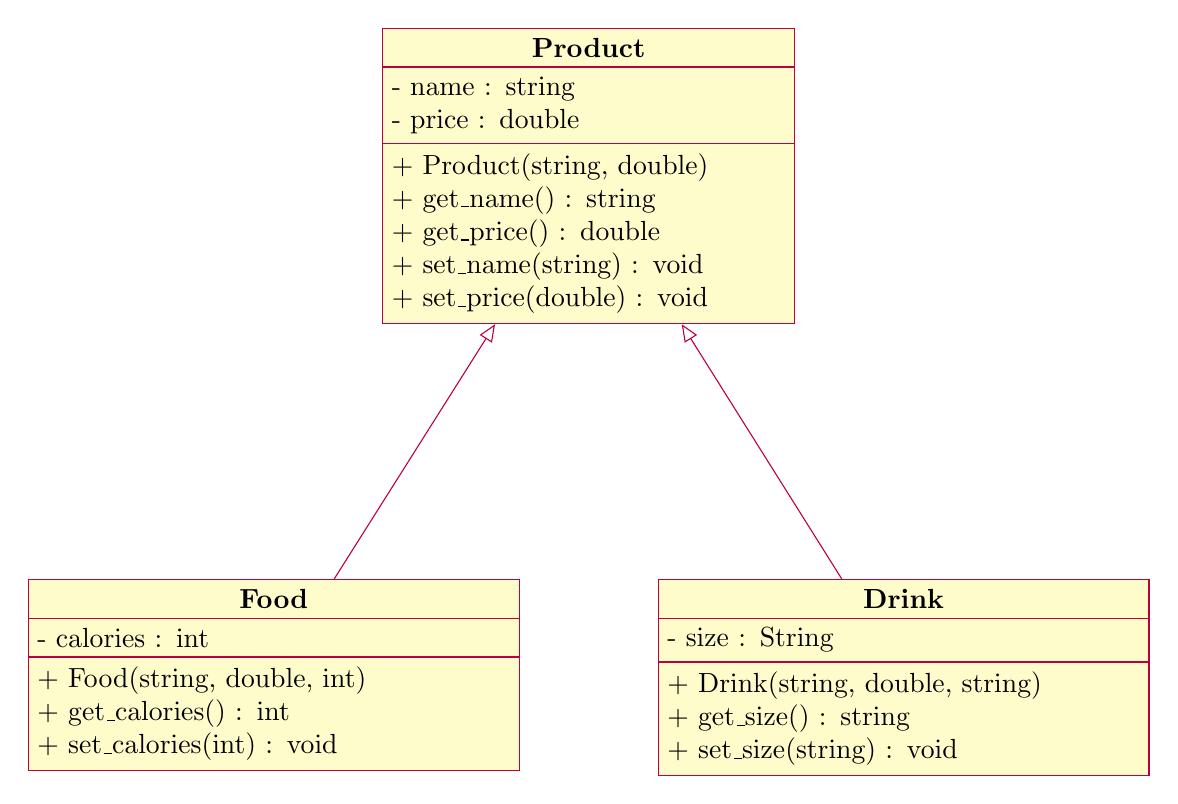
\begin{tikzpicture}
        \begin{class}[text width = 5cm]{Product}{0,0}
            \attribute{- name : string}
            \attribute{- price : double}
            \operation{+ Product(string, double)}
            \operation{+ get\_name() : string}
            \operation{+ get\_price() : double}
            \operation{+ set\_name(string) : void}
            \operation{+ set\_price(double) : void}
        \end{class}

        \begin{class}[text width = 6cm]{Food}{-4,-7}
            \inherit{Product}
            \attribute{- calories : int}
            \operation{+ Food(string, double, int)}
            \operation{+ get\_calories() : int}
            \operation{+ set\_calories(int) : void}
        \end{class}

        \begin{class}[text width = 6cm]{Drink}{4,-7}
            \inherit{Product}
            \attribute{- size : String}
            \operation{+ Drink(string, double, string)}
            \operation{+ get\_size() : string}
            \operation{+ set\_size(string) : void}
        \end{class}
    \end{tikzpicture}
    \caption{继承}
\end{figure}

产生继承关系后,子类可以通过调用父类中的属性和方法,也可以定义子类独有的属性和方法。\\

在创建子类对象时,会先调用父类的构造方法,然后再调用子类的构造方法。因此父类中必须存在一个构造方法,否则将无法创建子类对象。\\

\mybox{麦当劳}

\begin{lstlisting}[language=C++]
#ifndef _PRODUCT_H_
#define _PRODUCT_H_

#include <string>

class Product {
    protected:
    std::string name;
    double price;

    public:
    Product(std::string name, double price);
    std::string get_name();
    void set_name(std::string name);
    double get_price();
    void set_price(double price);
};

#endif
\end{lstlisting}

\begin{lstlisting}[language=C++]
#include "product.h"

Product::Product(std::string name, double price) {
    this->name = name;
    this->price = price;
}

std::string Product::get_name() {
    return name;
}

void Product::set_name(std::string name) {
    this->name = name;
}

double Product::get_price() {
    return price;
}

void Product::set_price(double price) {
    this->price = price;
}
\end{lstlisting}

\begin{lstlisting}[language=C++]
#ifndef _FOOG_H_
#define _FOOD_H_

#include <iostream>
#include <string>
#include "product.h"

class Food : public Product {
    private:
    int calories;

    public:
    Food(std::string name, double price, int calories);
    int get_calories();
    void set_calories(int calories);
    friend std::ostream& operator<<(std::ostream& os,
                                    const Food& food);
};

#endif
\end{lstlisting}

\begin{lstlisting}[language=C++]
#include "food.h"

Food::Food(std::string name, double price, int calories)
    : Product(name, price) {
    this->calories = calories;
}

int Food::get_calories() {
    return calories;
}

void Food::set_calories(int calories) {
    this->calories = calories;
}

std::ostream& operator<<(std::ostream& os, const Food& food) {
    os << "Food: " << food.name
       << " ($" << food.price << ") "
       << food.calories;
    return os;
}
\end{lstlisting}

\begin{lstlisting}[language=C++]
#ifndef _DRINK_H_
#define _DRINK_H_

#include <iostream>
#include <string>
#include "product.h"

class Drink : public Product {
    private:
    std::string size;

    public:
    Drink(std::string name, double price, std::string size);
    std::string get_size();
    void set_size(std::string size);
    friend std::ostream& operator<<(std::ostream& os,
                                    const Drink& drink);
};

#endif
\end{lstlisting}

\begin{lstlisting}[language=C++]
#include "drink.h"

Drink::Drink(std::string name, double price, std::string size)
    : Product(name, price) {
    this->size = size;
}

std::string Drink::get_size() {
    return size;
}

void Drink::set_size(std::string size) {
    this->size = size;
}

std::ostream& operator<<(std::ostream& os, const Drink& drink) {
    os << "Drink: " << drink.name
       << " ($" << drink.price << ") " 
       << drink.size;
    return os;
}
\end{lstlisting}

\begin{lstlisting}[language=C++]
#include <iostream>
#include "food.h"
#include "drink.h"

using namespace std;

int main() {
    Food food("Cheeseburger", 5.45, 302);
    Drink drink("Coke", 3.7, "Large");

    cout << food << endl;
    cout << drink << endl;

    return 0;
}
\end{lstlisting}

\begin{tcolorbox}
    \mybox{运行结果}
    \begin{verbatim}
Food: Cheeseburger ($5.45) 302
Drink: Coke ($3.7) Large
	\end{verbatim}
\end{tcolorbox}

\newpage

\section{抽象类}

\subsection{抽象类(Abstract Class)}

有些类只能用来做继承,不能用于创建对象。例如在动物园中并不存在“动物”这个对象,只有动物的子类对象,因此动物类不应该被实例化。\\

抽象类是一种不能被实例化的类,它用于定义接口或公共实现,供其它类继承并实现。

\vspace{-0.5cm}

\begin{lstlisting}[language=Java]
public abstract class Animal {}
\end{lstlisting}

\vspace{0.5cm}

\subsection{抽象方法}

有时候父类提供的方法无法满足子类不同的需求,但是如果不定义该方法,就表示该类具有该行为。\\

这种情况就可以将这个父类的方法定义为抽象方法,这样所有的子类都必须要重写该方法,否则子类仍然为抽象类。\\

抽象方法只需声明,而不用实现。包含抽象方法的类必须声明为抽象类。\\

\mybox{动物}

\begin{lstlisting}[language=Java]
public abstract class Animal {
    public abstract String sound();
}
\end{lstlisting}

\begin{lstlisting}[language=Java]
public class Dog extends Animal {
    @Override
    public String sound() {
        return "Woof";
    }
}
\end{lstlisting}

\begin{lstlisting}[language=Java]
public class Cat extends Animal {
    @Override
    public String sound() {
        return "Meow";
    }
}
\end{lstlisting}

\begin{lstlisting}[language=Java]
public class AnimalSound {
    public static void main(String[] args) {
        Dog dog = new Dog();
        Cat cat = new Cat();

        System.out.println("Dog's sound: " + dog.sound());
        System.out.println("Cat's sound: " + cat.sound());
    }
}
\end{lstlisting}

\begin{tcolorbox}
    \mybox{运行结果}
    \begin{verbatim}
Dog's sound: Woof
Cat's sound: Meow
	\end{verbatim}
\end{tcolorbox}

\newpage

\section{多态}

\subsection{多态(Polymorphism)}

多态是指对象可以具有多种形态,即同一个对象在不同时刻表现出不同的行为。例如Dog和Cat都是Animal的子类,因此可以将子类对象赋值给父类引用,从而产生多种形态。

\vspace{-0.5cm}

\begin{lstlisting}[language=Java]
Animal animal = new Dog();
\end{lstlisting}

由子类类型转型为父类类型,称为向上转型。由父类类型转型为子类类型,称为向下转型。\\

\mybox{员工工资}

\begin{lstlisting}[language=C++]
#ifndef _EMPLOYEE_H_
#define _EMPLOYEE_H_

#include <string>

class Employee {
    protected:
    std::string name;

    public:
    Employee(std::string name);
    std::string get_name();
    virtual double get_salary() = 0;
};

#endif
\end{lstlisting}

\begin{lstlisting}[language=C++]
#include "employee.h"

Employee::Employee(std::string name) {
    this->name = name;
}

std::string Employee::get_name() {
    return name;
}
\end{lstlisting}

\begin{lstlisting}[language=C++]
#ifndef _FULL_TIME_EMPLOYEE_H_
#define _FULL_TIME_EMPLOYEE_H_

#include "employee.h"

class FullTimeEmployee : public Employee {
    private:
    double basic_salary;
    double bonus;

    public:
    FullTimeEmployee(std::string name,
                     double basic_salary,
                     double bonus);
    virtual double get_salary() override;
};

#endif
\end{lstlisting}

\begin{lstlisting}[language=C++]
#include "full_time_employee.h"

FullTimeEmployee::FullTimeEmployee(std::string name,
                                    double basic_salary,
                                    double bonus)
        : Employee(name) {
    this->basic_salary = basic_salary;
    this->bonus = bonus;
}

double FullTimeEmployee::get_salary() {
    return basic_salary + bonus;
}
\end{lstlisting}

\begin{lstlisting}[language=C++]
#ifndef _PART_TIME_EMPLOYEE_H_
#define _PART_TIME_EMPLOYEE_H_

#include "employee.h"

class PartTimeEmployee : public Employee {
    private:
    double daily_wage;
    int working_days;

    public:
    PartTimeEmployee(std::string name,
                     double daily_wage,
                     int working_days);
    virtual double get_salary() override;
};

#endif
\end{lstlisting}

\begin{lstlisting}[language=C++]
#include "part_time_employee.h"

PartTimeEmployee::PartTimeEmployee(std::string name,
                                    double daily_wage,
                                    int working_days)
        : Employee(name) {
    this->daily_wage = daily_wage;
    this->working_days = working_days;
}

double PartTimeEmployee::get_salary() {
    return daily_wage * working_days;
}
\end{lstlisting}

\begin{lstlisting}[language=C++]
#include <iostream>
#include "full_time_employee.h"
#include "part_time_employee.h"

using namespace std;

int main() {
    Employee *employees[2] = {
        new FullTimeEmployee("Alice", 5783, 173),
        new PartTimeEmployee("Bob", 150, 15),
    };

    for (Employee *employee : employees) {
        cout << employee->get_name() << ": $"
             << employee->get_salary() << endl;
    }

    return 0;
}
\end{lstlisting}

\begin{tcolorbox}
    \mybox{运行结果}
    \begin{verbatim}
Alice: $5956
Bob: $2250
	\end{verbatim}
\end{tcolorbox}

\newpage

\end{document}